% !TeX spellcheck = russian-aot-ieyo
% Зачем: Определяет класс документа (То, как будет выглядеть документ)
% Примечание: параметр draft помечает строки, вышедшие за границы страницы, прямоугольником, в фильной версии его нужно удалить.
\documentclass[a4paper,14pt,russian,oneside,final,bibliography=totocnumbered]{extreport}


% Зачем: Установка кодировки исходных файлов.
\usepackage[utf8]{inputenc}

% Зачем: Делает результирующий PDF "searchable and copyable".
\usepackage{cmap}

% Зачем: Выбор внутренней TeX кодировки.
\usepackage[T2A]{fontenc}

% Зачем: Предоставляет свободный Times New Roman.
% Шрифт идёт вместе с пакетом scalable-cyrfonts-tex в Ubuntu/Debian
% раскомментировать, чтобы использовать scalable-cyrfonts-tex:
\usefont{T2A}{ftm}{m}{sl}

% Зачем: Чтобы можно было использовать русские буквы в формулах, но в случае использования предупреждать об этом.
\usepackage[warn]{mathtext}

% Зачем: Учет особенностей различных языков.
\usepackage[russian]{babel}

\usepackage[square,numbers,sort&compress]{natbib}
\setlength{\bibsep}{0em}

% Зачем: Перенос урлов на новую строку в позиции дефиса.
% hyperref импортирует url, поэтому задаем параметр неявно.
\PassOptionsToPackage{hyphens}{url}

\usepackage[final,hidelinks]{hyperref}

% Зачем: Подпись ссылок на рисунки вида "рисунок Х"
\addto\extrasrussian{%
  \def\figureautorefname{рисунок}%
}

\addto\captionsrussian{%
  % Зачем: Содержание пишется полужирным шрифтом, по центру всеми заглавными буквами
  % Почему: Пункт 2.2.7 Требований по оформлению пояснительной записки.
  \renewcommand\contentsname{\centerline{\bfseries\large{\MakeUppercase{содержание}}}}%
  % Зачем: Изменение надписи для списка литературы
  % Почему: Пункт 2.8.1 Требований по оформлению пояснительной записки.
  \renewcommand{\bibsection}{\sectioncentered*{Cписок использованных источников}}%
}

\AtEndDocument{%
  % Зачем: Добавление списка литературы в оглавление
  \addcontentsline{toc}{section}{Cписок использованных источников}%
}


% Зачем: Добавляет поддержу дополнительных размеров текста 8pt, 9pt, 10pt, 11pt, 12pt, 14pt, 17pt, and 20pt.
% Почему: Пункт 2.1.1 Требований по оформлению пояснительной записки.
\usepackage{extsizes}


% Зачем: Чтобы текст не вылазил за правую границу.
\sloppy


% Зачем: Типографские заморочки.
\usepackage{microtype}


% Зачем: Длинна, пимерно соответвующая 5 символам
% Почему: Требования содержат странное требование про отсупы в 5 символов (для немоноширинного шрифта :| )
\newlength{\fivecharsapprox}
\setlength{\fivecharsapprox}{6ex}


% Зачем: Добавляет отступы для абзацев.
% Почему: Пункт 2.1.3 Требований по оформлению пояснительной записки.
\usepackage{indentfirst}
\setlength{\parindent}{\fivecharsapprox} % Примерно соответсвует 5 символам.


% Зачем: Настраивает отступы от границ страницы.
% Почему: Пункт 2.1.2 Требований по оформлению пояснительной записки.
\usepackage[left=3cm,top=2.0cm,right=1.5cm,bottom=2.7cm]{geometry}


% Зачем: Настраивает межстрочный интервал, для размещения 40 +/- 3 строки текста на странице.
% Почему: Пункт 2.1.1 Требований по оформлению пояснительной записки.
\usepackage[nodisplayskipstretch]{setspace} 
\setstretch{1.1}
%\onehalfspacing

% Зачем: Выбор шрифта по-умолчанию. 
% Почему: Пункт 2.1.1 Требований по оформлению пояснительной записки.
% Примечание: В требованиях не указан, какой именно шрифт использовать. По традиции используем TNR.
\renewcommand{\rmdefault}{ftm} % Times New Roman


% Зачем: Отключает использование изменяемых межсловных пробелов.
% Почему: Так не принято делать в текстах на русском языке.
\frenchspacing


% Зачем: Сброс счетчика сносок для каждой страницы
% Примечание: в "Требованиях по оформлению пояснительной записки" не указано, как нужно делать, но в других БГУИРовских докуметах рекомендуется нумерация отдельная для каждой страницы
\usepackage{perpage}
\MakePerPage{footnote}


% Зачем: Добавляет скобку 1) к номеру сноски
% Почему: Пункты 2.9.2 и 2.9.1 Требований по оформлению пояснительной записки.
\makeatletter 
\def\@makefnmark{\hbox{\@textsuperscript{\normalfont\@thefnmark)}}}
\makeatother


% Зачем: Расположение сносок внизу страницы
% Почему: Пункт 2.9.2 Требований по оформлению пояснительной записки.
\usepackage[bottom]{footmisc}


% Зачем: Переопределяем стандартную нумерацию, т.к. в отчете будут только section и т.д. в терминологии TeX
\makeatletter
\renewcommand{\thesection}{\arabic{section}}
\makeatother


% Зачем: Пункты (в терминологии требований) в терминологии TeX subsubsection должны нумероваться
% Почему: Пункт 2.2.3 Требований по оформлению пояснительной записки.
\setcounter{secnumdepth}{3}


% Зачем: Настраивает отступ между таблицей с содержанимем и словом СОДЕРЖАНИЕ
% Почему: Пункт 2.2.7 Требований по оформлению пояснительной записки.
\usepackage{tocloft}
\setlength{\cftbeforetoctitleskip}{-1em}
\setlength{\cftaftertoctitleskip}{1em}


% Зачем: Определяет отступы слева для записей в таблице содержания.
% Почему: Пункт 2.2.7 Требований по оформлению пояснительной записки.
\makeatletter
\renewcommand{\l@section}{\@dottedtocline{1}{0.5em}{1.2em}}
\renewcommand{\l@subsection}{\@dottedtocline{2}{1.7em}{2.0em}}
\makeatother


% Зачем: Работа с колонтитулами
\usepackage{fancyhdr} % пакет для установки колонтитулов
\pagestyle{fancy} % смена стиля оформления страниц


% Зачем: Нумерация страниц располагается справа снизу страницы
% Почему: Пункт 2.2.8 Требований по оформлению пояснительной записки.
\fancyhf{} % очистка текущих значений
\fancyfoot[R]{\thepage} % установка верхнего колонтитула
\renewcommand{\footrulewidth}{0pt} % убрать разделительную линию внизу страницы
\renewcommand{\headrulewidth}{0pt} % убрать разделительную линию вверху страницы
\fancypagestyle{plain}{ 
    \fancyhf{}
    \rfoot{\thepage}}


% Зачем: Задает стиль заголовков раздела жирным шрифтом, прописными буквами, без точки в конце
% Почему: Пункты 2.1.1, 2.2.5, 2.2.6 и ПРИЛОЖЕНИЕ Л Требований по оформлению пояснительной записки.
\makeatletter
\renewcommand\section{%
  \clearpage\@startsection {section}{1}%
    {\fivecharsapprox}%
    {-1em \@plus -1ex \@minus -.2ex}%
    {1em \@plus .2ex}%
    {\raggedright\hyphenpenalty=10000\normalfont\large\bfseries\MakeUppercase}}
\makeatother


% Зачем: Задает стиль заголовков подразделов
% Почему: Пункты 2.1.1, 2.2.5 и ПРИЛОЖЕНИЕ Л Требований по оформлению пояснительной записки.
\makeatletter
\renewcommand\subsection{%
  \@startsection{subsection}{2}%
    {\fivecharsapprox}%
    {-1em \@plus -1ex \@minus -.2ex}%
    {1em \@plus .2ex}%
    {\raggedright\hyphenpenalty=10000\normalfont\normalsize\bfseries}}
\makeatother


% Зачем: Задает стиль заголовков пунктов
% Почему: Пункты 2.1.1, 2.2.5 и ПРИЛОЖЕНИЕ Л Требований по оформлению пояснительной записки.
\makeatletter
\renewcommand\subsubsection{
  \@startsection{subsubsection}{3}%
    {\fivecharsapprox}%
    {-1em \@plus -1ex \@minus -.2ex}%
    {\z@}%
    {\raggedright\hyphenpenalty=10000\normalfont\normalsize\bfseries}}
\makeatother

% Зачем: для оформления введения и заключения, они должны быть выровнены по центру.
% Почему: Пункты 1.1.15 и 1.1.11 Требований по оформлению пояснительной записки.
\makeatletter
\newcommand\sectioncentered{%
  \clearpage\@startsection {section}{1}%
    {\z@}%
    {-1em \@plus -1ex \@minus -.2ex}%
    {1em \@plus .2ex}%
    {\centering\hyphenpenalty=10000\normalfont\large\bfseries\MakeUppercase}%
    }
\makeatother



% Зачем: Задает стиль библиографии
% Почему: Пункт 2.8.6 Требований по оформлению пояснительной записки.
\bibliographystyle{styles/belarus-specific-utf8gost780u}


% Зачем: Пакет для вставки картинок
% Примечание: Объяснение, зачем final - http://tex.stackexchange.com/questions/11004/why-does-the-image-not-appear
\usepackage[final]{graphicx}
\DeclareGraphicsExtensions{.pdf,.png,.jpg,.eps}

% Зачем: Директория в которой будет происходить поиск картинок
\graphicspath{{figures/}}

% Зачем: Добавление подписей к рисункам
\usepackage{caption}
\usepackage{subcaption}

% Зачем: чтобы работала \No в новых латехах
\DeclareRobustCommand{\No}{\ifmmode{\nfss@text{\textnumero}}\else\textnumero\fi}

% Зачем: поворот ячеек таблиц на 90 градусов
\usepackage{rotating}
\DeclareRobustCommand{\povernut}[1]{\begin{sideways}{#1}\end{sideways}}


% Зачем: когда в формулах много кириллических символов команда \text{} занимает много места
\DeclareRobustCommand{\x}[1]{\text{#1}}


% Зачем: Задание подписей, разделителя и нумерации частей рисунков
% Почему: Пункт 2.5.5 Требований по оформлению пояснительной записки.
\DeclareCaptionLabelFormat{stbfigure}{Рисунок \emph{#2}}
\DeclareCaptionLabelFormat{stbtable}{Таблица \emph{#2}}
\DeclareCaptionLabelSeparator{stb}{~--~}
\captionsetup{labelsep=stb}
\captionsetup[figure]{labelformat=stbfigure,justification=centering}
\captionsetup[table]{labelformat=stbtable,justification=raggedright}
\renewcommand{\thesubfigure}{\asbuk{subfigure}}

% Зачем: Окружения для оформления формул
% Почему: Пункт 2.4.7 требований по оформлению пояснительной записки и специфические требования различных кафедр
% Пример использования смотри в course_content.tex, строка 5
\usepackage{calc}
\newlength{\lengthWordWhere}
\settowidth{\lengthWordWhere}{где}
\newenvironment{explanationx}
    {
    %%% Следующие строки определяют специфические требования разных редакций стандартов. Раскоменнтируйте нужную строку
    %% стандартный абзац, СТП-01 2010
    %\begin{itemize}[leftmargin=0cm, itemindent=\parindent + \lengthWordWhere + \labelsep, labelsep=\labelsep]

    %% без отступа, СТП-01 2013
    \begin{itemize}[leftmargin=0cm, itemindent=\lengthWordWhere + \labelsep , labelsep=\labelsep]

    \renewcommand\labelitemi{}
    }
    {
    \\[\parsep]
    \end{itemize}
    }

% Старое окружение для "где". Сохранено для совместимости
\usepackage{tabularx}

\newenvironment{explanation}
    {
    %%% Следующие строки определяют специфические требования разных редакций стандартов. Раскоменнтируйте нужные 2 строки
    %% стандартный абзац, СТП-01 2010
    %\par 
    %\tabularx{\textwidth-\fivecharsapprox}{@{}ll@{ --- } X }
    %% без отступа, СТП-01 2013
    \noindent 
    \tabularx{\textwidth}{@{}ll@{ --- } X }
    }
    { 
    \\[\parsep]
    \endtabularx
    }


% Зачем: Удобная вёрстка многострочных формул, масштабирующийся текст в формулах, формулы в рамках и др
\usepackage{amsmath}


% Зачем: Поддержка ажурного и готического шрифтов 
\usepackage{amsfonts}


% Зачем: amsfonts + несколько сотен дополнительных математических символов
\usepackage{amssymb}


% Зачем: Окружения «теорема», «лемма»
\usepackage{amsthm}


% Зачем: Производить арифметические операции во время компиляции TeX файла
\usepackage{calc}

% Зачем: Производить арифметические операции во время компиляции TeX файла
\usepackage{fp}

% Зачем: Пакет для работы с перечислениями
\usepackage{enumitem}
\makeatletter
 \AddEnumerateCounter{\asbuk}{\@asbuk}{щ)}
\makeatother


% Зачем: Устанавливает символ начала простого перечисления
% Почему: Пункт 2.3.5 Требований по оформлению пояснительной записки.
\setlist{nolistsep}


% Зачем: Устанавливает символ начала именованного перечисления
% Почему: Пункт 2.3.8 Требований по оформлению пояснительной записки.
\renewcommand{\labelenumi}{\asbuk{enumi})}
\renewcommand{\labelenumii}{\arabic{enumii})}

% Зачем: Устанавливает отступ от границы документа до символа списка, чтобы этот отступ равнялся отступу параграфа
% Почему: Пункт 2.3.5 Требований по оформлению пояснительной записки.

\setlist[itemize,0]{itemindent=\parindent + 2.2ex,leftmargin=0ex,label=--}
\setlist[enumerate,1]{itemindent=\parindent + 2.7ex,leftmargin=0ex}
\setlist[enumerate,2]{itemindent=\parindent + \parindent - 2.7ex}

% Зачем: Включение номера раздела в номер формулы. Нумерация формул внутри раздела.
\AtBeginDocument{\numberwithin{equation}{section}}

% Зачем: Включение номера раздела в номер таблицы. Нумерация таблиц внутри раздела.
\AtBeginDocument{\numberwithin{table}{section}}

% Зачем: Включение номера раздела в номер рисунка. Нумерация рисунков внутри раздела.
\AtBeginDocument{\numberwithin{figure}{section}}


% Зачем: Дополнительные возможности в форматировании таблиц
\usepackage{makecell}
\usepackage{multirow}
\usepackage{array}


% Зачем: "Умная" запятая в математических формулах. В дробных числах не добавляет пробел
% Почему: В требованиях не нашел, но в русском языке для дробных чисел используется {,} а не {.}
\usepackage{icomma}

% Зачем: Печать римских чисел.
\usepackage{romannum}


% Зачем: Символы для siunitx в T1 кодировке
\usepackage{textcomp}

% Зачем: Управление выводом чисел.
\usepackage{siunitx}
\sisetup{output-decimal-marker = {,}}

% Зачем: inline-коментирование содержимого.
\newcommand{\ignore}[2]{\hspace{0in}#2}


% Зачем: Возможность коментировать большие участки документа
\usepackage{verbatim}


\usepackage{xcolor}


% Зачем: Оформление листингов кода
% WARNING: необходима версия 2.0+
\usepackage{minted}

% Зачем: Нумерация листингов в пределах секции
%\AtBeginDocument{\numberwithin{lstlisting}{section}}

\usepackage[normalem]{ulem}

% Моноширинный шрифт выглядит визуально больше, чем пропорциональный шрифт, если их размеры одинаковы. Искусственно уменьшаем размер ссылок.
\renewcommand{\UrlFont}{\small\rmfamily\tt}

% Магия для подсчета разнообразных объектов в документе
\usepackage{lastpage}
\usepackage{totcount}
\regtotcounter{section}

\usepackage{etoolbox}

\newcounter{totfigures}
\newcounter{tottables}
\newcounter{totreferences}
\newcounter{totequation}

\providecommand\totfig{} 
\providecommand\tottab{}
\providecommand\totref{}
\providecommand\toteq{}

\makeatletter
\AtEndDocument{%
  \addtocounter{totfigures}{\value{figure}}%
  \addtocounter{tottables}{\value{table}}%
  \addtocounter{totequation}{\value{equation}}
  \immediate\write\@mainaux{%
    \string\gdef\string\totfig{\number\value{totfigures}}%
    \string\gdef\string\tottab{\number\value{tottables}}%
    \string\gdef\string\totref{\number\value{totreferences}}%
    \string\gdef\string\toteq{\number\value{totequation}}%
  }%
}
\makeatother

\pretocmd{\section}{\addtocounter{totfigures}{\value{figure}}\setcounter{figure}{0}}{}{}
\pretocmd{\section}{\addtocounter{tottables}{\value{table}}\setcounter{table}{0}}{}{}
\pretocmd{\section}{\addtocounter{totequation}{\value{equation}}\setcounter{equation}{0}}{}{}
\pretocmd{\bibitem}{\addtocounter{totreferences}{1}}{}{}



% Для оформления таблиц не влязящих на 1 страницу
\usepackage{longtable}

% Для включения pdf документов в результирующий файл
\usepackage{pdfpages}

% Для использования знака градуса и других знаков
% http://ctan.org/pkg/gensymb
\usepackage{gensymb}

% Зачем: преобразовывать текст в верхний регистр командой MakeTextUppercase
\usepackage{textcase}

% Зачем: Переносы в словах с тире.
% Тире в словае заменяем на \hyph: аппаратно\hyphпрограммный.
% https://stackoverflow.com/questions/2193307/how-to-get-latex-to-hyphenate-a-word-that-contains-a-dash#
\def\hyph{-\penalty0\hskip0pt\relax}

% Добавляем левый отступ для библиографии
% https://tex.stackexchange.com/questions/133253/leftmargin-problem-at-the-bibliography
\makeatletter
\renewenvironment{thebibliography}[1]
     {\sectioncentered*{Cписок использованных источников}
      \@mkboth{\MakeUppercase\refname}{\MakeUppercase\refname}%
      \list{\@biblabel{\@arabic\c@enumiv}}%
           {\settowidth\labelwidth{\@biblabel{#1}}%
            \setlength{\itemindent}{\dimexpr\labelwidth+\labelsep+1em}
            \leftmargin\z@
            \@openbib@code
            \usecounter{enumiv}%
            \let\p@enumiv\@empty
            \renewcommand\theenumiv{\@arabic\c@enumiv}}%
      \sloppy
      \clubpenalty4000
      \@clubpenalty \clubpenalty
      \widowpenalty4000%
      \sfcode`\.\@m}
     {\def\@noitemerr
       {\@latex@warning{Empty `thebibliography' environment}}%
      \endlist}
\makeatother

% Макросы
\newcommand{\csharp}{C\#}
\newcommand{\fsharp}{F\#}
\newcommand{\vbnet}{Visual Basic~.NET}
\newcommand{\cpp}{C\texttt{\hspace{-0.3ex}+\hspace{-0.25ex}+}}
\newcommand{\cppcli}{Visual \cpp{}/CLI}
\newcommand{\dotnet}{Microsoft .NET}
\newcommand{\netfx}{.NET Framework}
\newcommand{\java}{Java}
\newcommand{\python}{Python}
\newcommand{\django}{Django}
\newcommand{\purec}{C}
\newcommand{\sdr}{Software Defined Radio}
\newcommand{\SDR}{SDR}
\listfiles


\begin{document}

\begin{titlepage}
  \begin{center}
    Министерство образования Республики Беларусь\\[1em]
    Учреждение образования\\
    БЕЛОРУССКИЙ ГОСУДАРСТВЕННЫЙ УНИВЕРСИТЕТ \\
    ИНФОРМАТИКИ И РАДИОЭЛЕКТРОНИКИ\\[1em]

    \begin{minipage}{\textwidth}
      \begin{flushleft}
        \begin{tabular}{ l l }
          Факультет & Компьютерных систем и сетей\\
          Кафедра   & Информатики
        \end{tabular}
      \end{flushleft}
    \end{minipage}\\[1em]

    \begin{minipage}{\textwidth}
      \begin{flushright}
        \textit{К защите допустить:}\\
        Заведующий кафедрой информатики\\
        \underline{\hspace*{4.5cm}} Н.\,А.~Волорова
      \end{flushright}
    \end{minipage}\\[3em]

    {ПОЯСНИТЕЛЬНАЯ ЗАПИСКА}\\
    {к дипломному проекту}\\
    {на тему:}\\[1em]
    \textbf{\large ПРОГРАММНОЕ СРЕДСТВО ДЛЯ ОБНАРУЖЕНИЯ РАДИОСИГНАЛОВ С ПОМОЩЬЮ SDR-ПРИЕМНИКА}\\[1em]


    {БГУИР ДП \textbf{1-31 03 04 07 093} ПЗ}\\[2em]
    
    \begin{tabular}{ p{0.65\textwidth}p{0.25\textwidth} }
      Студент: & А.\,А.~Михолап \\
      Руководитель: & М.\,В.~Стержанов \\
      Консультанты: &\\
      \hspace*{3ex}\emph{от кафедры информатики} & М.\,В.~Стержанов \\
      \hspace*{3ex}\emph{по экономической части} & К.\,Р.~Литвинович \\
      \hspace*{3ex}\emph{по охране труда} & Т.\,В.~Гордейчук \\
      Нормоконтролёр: & С.\,И.~Сиротко\\
      \\
      Рецензент: &
    \end{tabular}
    
    \vfill
    {\normalsize Минск 2015}
  \end{center}
\end{titlepage}
 % page 1

\sectioncentered*{Реферат}
\thispagestyle{empty}

\emph{Ключевые слова}: \MakeUppercase{software-defined radio; цифровая обработка сигналов; обнаружение сигналов; спектральный анализ сигналов; моделирование случайных процессов}.

\vspace{4\parsep}

Дипломный проект выполнен на 6 листах формата А1 с пояснительной запиской на~\pageref*{LastPage} страницах, без приложений справочного или информационного характера. 
Пояснительная записка включает \total{section}~глав, \totfig{}~рисунков, \tottab{}~таблиц, \toteq{}~формул и \totref{}~литературный источник.

Целью дипломного проекта является разработка программного средства, использующего аппаратное обеспечение software defined radio для сканирования радиоэфира и обнаружения нешумовых сигналов.

Для достижения цели дипломного проекта было разработано прикладное программное средство на языках \python{} и \purec{}, работающее в режиме сканирования радиоэфира, а также пользовательский интерфейс для интерактивной работы.
Приложение использует методы математической статистики и математического моделирования для обнаружения различных видов радиосигналов.

В разделе технико-экономического обоснования был произведён расчёт затрат на создание ПО, а также прибыли от разработки, получаемой разработчиком.
Проведённые расчёты показали экономическую целесообразность проекта.

Пояснительная записка включает раздел по охране труда, в котором была произведена оценка пожарной безопасности на предприятии, где была пройдена преддипломная практика.

\clearpage
 % page 2

%{
  \newgeometry{top=1.25cm,bottom=1.25cm,right=1cm,left=2cm,twoside}
  \thispagestyle{empty}
  \setlength{\parindent}{0em}

  \newcommand{\lineunderscore}{\uline{\hspace*{\fill}}}
  \newcommand{\underlined}[1]{\uline{ #1\hfill}}
  \newcommand{\underlinedbox}[2]{\makebox[#1]{\uline{ #2\hfill}}}
  \newcommand{\underlinedcentered}[1]{\centering\uline{\makebox[\linewidth]{#1}}}

  \begin{center}
    Министерство образования Республики Беларусь\\
    Учреждение образования\\
    БЕЛОРУССКИЙ ГОСУДАРСТВЕННЫЙ УНИВЕРСИТЕТ \\
    ИНФОРМАТИКИ И РАДИОЭЛЕКТРОНИКИ\\[1em]


  \begin{minipage}{\textwidth}
    \begin{flushleft}
      \begin{tabular}{ p{0.20\textwidth}p{0.31\textwidth}p{0.20\textwidth}p{0.20\textwidth} @{} }
        Факультет & \underlined{КСиС} & Кафедра & \underlined{Информатики} \\
        Специальность & \underlined{1-31 03 04} & Специализация & \underlined{07}
      \end{tabular}
    \end{flushleft}
  \end{minipage}\\[1em]

  \begin{minipage}{\textwidth}
    \begin{flushright}
      \begin{tabular}{p{0.40\textwidth}}
        \hspace{6.8em} УТВЕРЖДАЮ \\
        \underline{\hspace*{7em}} Зав. кафедрой \\
        <<\underline{\hspace*{4ex}}>> \underline{\hspace*{7em}} 2015 г.
      \end{tabular}
    \end{flushright}
  \end{minipage}\\[1em]

  \textbf{ЗАДАНИЕ} \\
  \textbf{по дипломному проекту (работе) студента}

  \underlinedcentered{Михолапа Алеся Александровича}\\
  {\small (фамилия, имя, отчество) }

  \end{center}

  \vspace{1em}

  1. Тема проекта (работы):
  \underlined{Программное средство для обнаружения радиосигналов с помощью \SDR-приемника} \\
  утверждена приказом по университету от <<\underlinedbox{1.5em}{25}>> \underlinedbox{5em}{марта} 2015 г. \No{} \underlined{510-с}

  \vspace{1em}

  2. Срок сдачи студентом законченного проекта (работы): \lineunderscore

  \vspace{1em}

  3. Исходные данные к проекту (работе):
  \underlined{Назначение разработки: создать программный радиосканер на аппаратной основе \sdr, способный обнаруживать нешумовые сигналы в исследуемой полосе частот.}\\
  \lineunderscore

  \vspace{1em}

  4. Содержание пояснительной записки (перечень подлежащих разработке вопросов):
  \underlined{Введение}\\
  \underlined{1 Обзор предметной области}\\
  \underlined{2 Аппаратное обеспечение}\\
  \underlined{3 Методы обнаружения сигналов}\\
  \underlined{4 Описание разработанных алгоритмов}\\
  \underlined{5 Технико-экономическое обоснование}\\
  \underlined{6 Обеспечение пожарной безопасности на предприятии}\\
  \underlined{Заключение}

  \clearpage
  \thispagestyle{empty}

  5. Перечень графического материала (с точным указанием обязательных чертежей):
  \underlined{Последовательность обработки сигнала (ПД1) - формат А1, лист 1}\\
  \underlined{Блок-схема алгоритма обнаружения WFM сигналов (ПД2) - формат А1, лист 1}\\
  \underlined{Блок-схема алгоритма обнаружения NFM сигналов (ПД3) - формат А1, лист 1}\\
  \underlined{\SDR-приемники (ПЛ1) - формат А1, лист 1}\\
  \underlined{Спектрограммы различных типов сигналов (ПЛ2) - формат А1, лист 1}\\
  \underlined{Суточная спектрограмма широкого диапазона частот (ПЛ3) - формат А1, лист 1}\\

  \vspace{1em}

  6. Содержание задания по технико-экономическому обоснованию.\\
  \underlined{Расчет экономической эффективности от продажи разработанного программного продукта}\\
  \lineunderscore

  Задание выдал \hspace{1em} \uline{\hspace*{6em}} \hspace{1em} К.\,Р.~Литвинович

  \vspace{1em}

  7. Содержание задания по охране труда.\\
  \underlined{Обеспечение пожарной безопасности на предприятии <<ЯндексБел>>}\\
  \lineunderscore

  Задание выдал \hspace{1em} \uline{\hspace*{6em}} \hspace{1em} Т.\,В.~Гордейчук

  \vfill

  \begin{center}
    КАЛЕНДАРНЫЙ ПЛАН
  \end{center}

  \begingroup
  \small
  \begin{tabular}{| >{\centering}m{0.04\textwidth} 
                  | >{\centering}m{0.40\textwidth} 
                  | >{\centering}m{0.08\textwidth}
                  | >{\centering}m{0.19\textwidth}  
                  | >{\centering\arraybackslash}m{0.16\textwidth}|}
    \hline \No{} п/п & Наименование этапов дипломного проекта (работы) & Объем этапа, \% & Срок выполнения этапов & Примечание \\
    \hline 1 & Изучение материалов о предметной области & 10-15 & 25.01 - 15.02& \\
    \hline 2 & Поиск аналогов, формулирование конкретных задач & 10 & 16.02 - 28.02 & \\
    \hline 3 & Расчет экономической эффективности и выполнение задания по охране труда & 15-20 & 01.03 - 20.03 & \\
    \hline 4 & Создание прототипа, исследование различных алгоритмов & 20 & 21.03 - 15.04 & \\
    \hline 5 & Конечная реализация разработанных методов & 15-20 & 16.04 - 10.05 & \\
    \hline 6 & Оформление пояснительной записки и графического материала & 20-25 & 11.05 - 01.06 & \\
    \hline
  \end{tabular}
  \endgroup

  \vspace{2em}

  Дата выдачи задания: \uline{\hspace*{6em}} \hspace{2ex} Руководитель \hfill{} \uline{\hspace*{4em}} М.\,В.~Стержанов

  \vspace{1em}

  Задание принял к исполнению \hfill{} \uline{\hspace*{4em}} А.\,А.~Михолап

  \restoregeometry
}
 % pages 3 and 4. printed separately

%\sectioncentered*{Аннотация}
\thispagestyle{empty}

\begin{center}
  \begin{minipage}{0.82\textwidth}
    на дипломный проект <<Программное средство для обнаружения радиосигналов с помощью SDR-приемника>> студента УО <<Белорусский государственный университет информатики и радиоэлектроники>> Михолапа~А.\,А.
  \end{minipage}
\end{center}

\emph{Ключевые слова}: \MakeUppercase{software-defined radio; цифровая обработка сигналов; обнаружение сигналов; спектральный анализ сигналов; моделирование случайных процессов}.

\vspace{4\parsep}

Дипломный проект выполнен на 6 листах формата А1 с пояснительной запиской на~\pageref*{LastPage} страницах, без приложений справочного или информационного характера. 
Пояснительная записка включает \total{section}~глав, \totfig{}~рисунка, \tottab{}~таблиц, \toteq{}~формулы, \totref{}~литературных источников.

Целью дипломного проекта является разработка радиосканера на аппаратной базе \sdr, способного производить пассивное сканирование эфира и оповещать о присутствии в нем активных каналов передачи.

Для достижения цели дипломного проекта было разработано программное средство, способное обнаружать нешумовые сигналы в заданной полосе частот.

Во введении происходит ознакомление с проблемой, решаемой в дипломном проекте и кратко описываются отличия \SDR\ от традиционных радиосредств.

В первой главе производится обзор предметной области --- основных типов сигналов и помех и математических конструкций, применяемых в задачах обнаружения сигналов.

Во второй главе детальнее рассказывается об особенностях \SDR, его технических характеристиках и основных принципах работы.

В третьей главе приводятся математические алгоритмы, использованные в дипломном проекте.

В четвертой главе описывается реализация программного продукта.

В пятой главе производится технико"=экономическое обоснование разработки.

В шестой главе производится оценка пожарной безопасности предприятия, на котором была пройдена преддипломная практика.

В заключении подводятся итоги и делаются выводы по дипломному проекту, а также описывается дальнейший план развития проекта.

\clearpage
 % not part of report

%\thispagestyle{empty}

\begin{singlespace}

{\small
  \begin{center}
    \begin{minipage}{0.8\textwidth}
      \begin{center}
        {\normalsize ОТЗЫВ}\\[1em]
        на дипломный проект студента факультета компьютерных систем и сетей 
        Учреждения образования <<Белорусский государственный университет информатики и радиоэлектроники>>\\
        Михолапа Алеся Александровича \\
        на тему: <<Программное средство для обраружения радиосигналов с помощью \SDR-приемника>>
      \end{center}
    \end{minipage}
  \end{center}

Целью дипломного проекта Михолапа А.А. было создание радиосканера на аппаратной основе \sdr.
В настоящее время наблюдается рост популярности \SDR. Предпринимаются первые шаги по применению этих систем для решения открытых задач радиотехники, таких как обеспечение электромагнитной совместимости радиосредств и возможность модификации их характеристик без изменения аппаратной базы.
Исследования в этом направлении имеют перспективы найти практическое применение в современной радиотехнике.

Выбранная тема разработки программного продукта глубоко пересекается с непрофильными для студентов факультета компьютерных систем и сетей областями цифровой обработки сигналов и радиосвязи. Михолап А.А. самостоятельно изучил специализированную литературу на достаточно глубоком уровне и продемонстрировал способность использовать приобретенные навыки в новой предметной области.

В разработанном приложении применены широко используемые в профессиональной среде технологии программирования, а продуманная архитектура подходит для наращивания функциональности и дальнейшего развития.
Реализованные алгоритмы используют достижения различных прикладных наук: цифровой обработки сигналов, статистики, математического моделирования.

Календарный график в процессе выполнения задания не нарушался. На всех точках контроля объем проделанной работы соответствовал ожидаемому.

Пояснительная записка написана точно, последовательно, со всесторонним пониманием темы. Она содержит необходимые знания о предметной области и полно освещает методы, подходы и инструменты, использованные для решения задачи.
Пояснительная записка и графический материал оформлены в соответствии с требованиями ЕСКД.

Продемонстрированный Михолапом А.А. уровень профессиональной подготовки и способность самостоятельно осваивать новые области знания позволяют считать цель его обучения достигнутой, а его самого достоиным присвоения квалификации математик-системный программист.

  \vfill
  \noindent
  \begin{minipage}{0.54\textwidth}
    \begin{flushleft}
      Руководитель проекта:\\
      кандитат технических наук, доцент,\\
      доцент кафедры информатики\\[0.2em]
      27.05.15
    \end{flushleft}
  \end{minipage}
  \begin{minipage}{0.44\textwidth}
    \begin{flushright}
      \underline{\hspace*{3cm}} М.\,В.~Стержанов
    \end{flushright}
  \end{minipage}
}

\end{singlespace}

\clearpage
 % not part of report

%\thispagestyle{empty}


{\small
  \begin{center}
    \begin{minipage}{0.9\textwidth}
      \begin{center}
        {\normalsize РЕЦЕНЗИЯ}\\[0.2cm]
        на дипломный проект студента факультета компьютерных систем и сетей Учреждения образования <<Белорусский государственный университет информатики и радиоэлектроники>>\\
        Михолапа Алеся Александровича \\
        на тему: <<Программное средство для обнаружения радиосигналов с помощью \SDR-приемника>>
      \end{center}
    \end{minipage}\\
  \end{center}

Дипломный проект студента Михолапа А.А. состоит из шести листов графического материала и~\pageref*{LastPage} страниц пояснительной записки.

Темой проекта выбрано применение программируемого радиоприемника в задаче обнаружения сигналов.
В настоящее время этот тип устройств находится на стадии экспериментального внедрения в различные сферы радиотехники, что говорит о перспективности разработок на его основе.

В пояснительной записке собраны все необходимые сведения по теоретическому обоснованию и практической реализации проекта.
Приведенный материал позволяет получить целостное восприятие проблемы и способов ее решения.
Большое количество иллюстраций гармонично дополняет текст и способствует лучшему пониманию изложенных идей.

Дано описание технических характеристик и принципов работы \sdr.
Произведен обзор предметной области, описаны математические конструкции для представления радиосигналов и различные алгоритмы их обработки.
Подробно изложена архитектура программного средства и реализованные методы обнаружения.

Предложены различные пути решения проблемы, использующие в своей основе математическое моделирование и статистику.
Логично и обоснованно проанализированы их преимущества и недостатки, рассмотрены дальнейшие пути развития проекта.
Разностороннее и подробное изложение свидетельствует об интенсивной работе с литературными источниками из разных областей математики и информатики.

Пояснительная записка и графический материал оформлены аккуратно и в соответствии с требованиями ЕСКД.

Созданное программное средство может использоваться как часть радиотехнической системы.
Предусмотрено расширение функциональности продукта через систему модулей для поддержки новых типов сигналов.

Замечания:
\begin{itemize}
  \item{при сравнении аппаратных средств не указана стабильность частоты;}
  \item{при описании реализации не указан использованный тип окна для оконного преобразования Фурье.}
\end{itemize}

Дипломный проект полно раскрывает обозначенную тему, демонстрирует умение осваивать и работать с современными технологиями и заслуживает оценки десять баллов, а дипломник Михолап А.А. --- присвоения квалификации математик-системный программист.

  \vfill
  \noindent
  \begin{minipage}{0.4\textwidth}
    \begin{flushleft}
      Рецензент:\\
      Преподаватель 1 к. каф. информатики УО\\
      «Минский государственный высший радиотехнический колледж»
    \end{flushleft}
  \end{minipage}
  \begin{minipage}{0.58\textwidth}
    \begin{flushright}
    \underline{\hspace*{3cm}}\hspace*{0.5cm}\underline{\hspace*{2cm}} С.\,Г.~Буянова \\
    Дата\hspace*{6.5cm}
    \end{flushright}
  \end{minipage}
}

\clearpage
 % not part of report

\setcounter{page}{5}

% Зачем: Содержание пишется полужирным шрифтом, по центру всеми заглавными буквами
% Почему: Пункт 2.2.7 Требований по оформлению пояснительной записки.
\renewcommand \contentsname {\centerline{\bfseries\large{\MakeUppercase{содержание}}}}

% Зачем: Не захламлять основной файл
% Примечание: \small\selectfont злостный хак, чтобы уменьшить размер шрифта в ToC 
{
\normalsize\selectfont
\tableofcontents
\newpage
}

\sectioncentered*{Введение}
\addcontentsline{toc}{section}{Введение}
\label{sec:intro}

В 1886 году Генрих Герц открыл существование электромагнитных волн, а уже через 20 лет с их помощью научились передавать информацию. Так началась эпоха радиосвязи, которая подолжается и в наши дни. Связь без проводов прочно вошла в жизни огромного множества людей, от моряков, получивших возможность общаться с сушей, до большинства из нас, как пользователей мобильных телефонов. Анализ радиоизлучения позволил определять расположение удаленных объектов и даже понять из чего сделаны звезды. Открытие Герца, можно сказать, дало человечеству новый орган восприятия, значительно усиливший потенциал его возможностей.

Традиционно тракт приема и передачи сигнала полностью реализуется в электронных схемах. Для каждой операции --- фильтр, модуляция, демодуляция и пр. --- существует свой физический компонент. Составляя их в последовательности можно получить самые разнообразные функциональные элементы. Такой подход успешно применяется на практике, но он накладывает определенные ограничения на использование и поддержку таких систем. Однажды спроектированная и построенная, она не может изменить свои характеристики в процессе эксплуатации, или изменяет их заранее продуманным способом. Это означает, что старый приемник не сможет обрабатывать новый вид сигналов, а в собранную рацию нельзя добавить новый криптографический алгоритм.

Такое положение вещей было оспорено к концу \Romannum{19} века, когда начались попытки внести гибкость программного обеспечения в мир радиоэлектроники. Функции некоторых элементов приемопередающего тракта воплотили в виде программных компонент. Эта инициатива была поддержана военными США, которые в 1990г. запустили первый публичный проект по внедрению \SDR --- SPEAKeasy \cite{speakeasy_wiki}. Их целью было создание копий существующих раций, которые смогли бы поддерживать новые стандарты связи.

Долгое время оборудование для радиосвязи, особенно нетрадиционные \SDR, стоило достаточно больших денег. Но в последние годы радиолюбители обнаружили, что с помощью платы дешевого DVB-T TV тюнера можно получать радиосигнал в комплексной форме, а значит использовать его как радиоприемник \cite{rtl_sdr_about}. Конечно, качество приема значительно отстает от профессиональных средств, а передатчика в комплекте нет вообще, но это позволило любому желающему проводить свои эксперименты в радиоэфире. В работе используется \SDR-приемник именно такого типа.

Целью дипломного проекта было выбрано обнаружение сигналов. Это фундаментальная задача во многих областях радиотехники, от проектирования любительских радиоприемников до радиоразведки. Теоретические принципы и методы в этом направлении хорошо исследованы, интерес представляет их практическое применение для широкого класса сигналов с использованием \sdr.

В рамках проекта будет создано программное средство, способное сканировать заданную полосу частот и выделять в ней области присутствия нешумовых сигналов. В качестве радиоприемного устройства используется R820T/R820T2 RTL-SDR. Цифровая обработка сигналов реализована на языке программирования Python. При анализе применены методы математической статистики.

В первой главе говорится об аналогах данного программного средства и его отличиях. Далее дается описание аппаратной части проекта, технические характеристики, возможности и ограничения платформы. В следующей главе объясняется выбор использованных математических методов. Завершает основную часть обзор результатов применения приложения.


\section{Обзор предметной области}
\label{sec:domain}

\subsection{Математическое понимание радиосигнала (1)}

Радиосвязь --- это разновидность беспроводной связи, где носителем сигнала является радиоволна. Передача и прием информации осуществляется посредством излучения и поглощения электромагнитных колебаний.
Передаваемые данные как правило неслучайны и могут быть представлена как функция от полезной информации и времени. В идеальных условиях было бы возможно, имея некоторые априорные знания о характере сигнала, безошибочно восстановить эту функцию и получить полезную информацию без потерь. Для примера можно рассмотреть стандартную запись сигнала с фазовой модуляцией (\autoref{eq:domain:pm_example}).

\begin{equation}
  \label{eq:domain:pm_example}
  s(t) = A_0 cos(\omega_0 t + m s_m(t))
\end{equation}
\begin{explanation}
\item[где] $s_m(t)$ --- полезная информация.
\end{explanation}

Но при распространении электромагнитной волны, она неизбежно испытывает влияние среды и изменяет свои параметры. Кроме того, вместе с целевым сигналом на приемник поступают множество шумовых. В результате полезную информацию можно восстановить только с определенной погрешностью.
Мгновенный уровень сигнала при этом непредсказуемо колеблется, поэтому в каждый момент времени его можно рассматривать как реализацию некоторой случайной величины, а развернутый во времени сигнал как случайный процесс. Такая абстракция очень полезна при статистическом анализе сигнала, так как позволяет использовать известные математические приемы при исследовании. Кроме того, его неизбежная составляющая --- фоновый шум --- обычно имеет нормальное распределение с нулевым математическим ожиданием.

Эта математическая модель обобщается на случай смесей сигналов и разладок (изменений параметров предполагаемого распределения). Также над случайными величинами определены математические операции: сложение, умножение и др. Это значит, что в терминах случайного процесса воспроизводимы как минимум элементарные преобразования сигналов.

\subsection{Типы сигналов (3)}

Полезная информация, передаваемая средствами радиосвязи имеет произвольные параметры и не годится для непосредственного использования как сигнал. Сначала она должна быть преобразована к желаемой полосе частот. Этот принцип позволяет использовать радио эфир с наибольшей эффективностью --- каждый передатчик работает на своей частоте и не мешает соседям.

Сигнал, заключенный в целевую полосу частот называется несущим, полезный сигнал --- модулирующим, а процесс кодирования модулирующего в несущий --- модуляцией. Для того применять методы их обнаружения необходимо понимать особенности встречаемых типов модуляции.


\subsubsection{Модулирующий сигнал.}\ В следующих пунктах будут рассмотрены характеристики различных способов модуляции. Чтобы ясно увидеть их отличия, зафиксируем модулирующий сигнал. Он был получен смесью трех синусоид с различными частотами и начальными фазами.

\begin{figure}[h]
  \centering
  \begin{subfigure}{0.45\textwidth}
    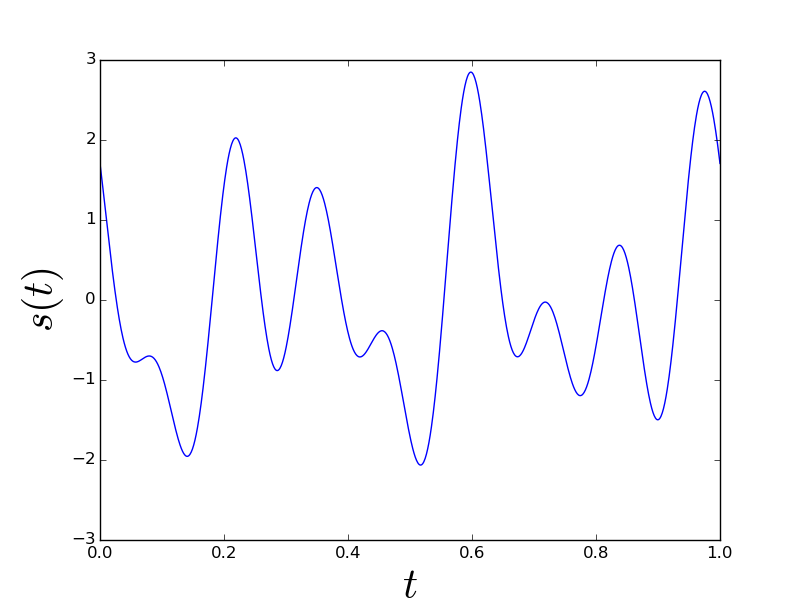
\includegraphics[width=\textwidth]{domain/modulator_example_time}
    \caption{}
  \end{subfigure}
  \begin{subfigure}{0.45\textwidth}
    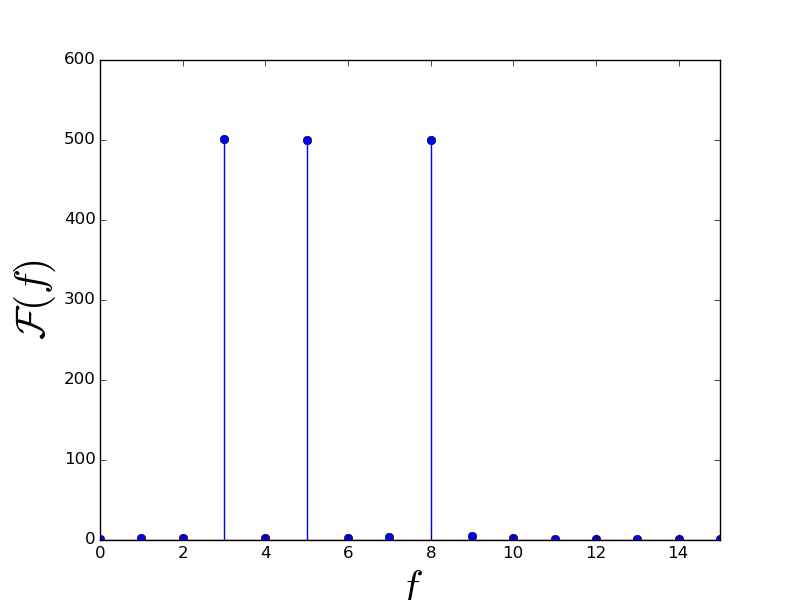
\includegraphics[width=\textwidth]{domain/modulator_example_freq}
    \caption{}
  \end{subfigure}
  \caption{Временная (а) и частотная (б) диаграммы модулирующего сигнала}
  \label{fig:domain:modulator}
\end{figure}

\subsubsection{Амплитудная модуляция (AM).}\ Амплитуда несущего сигнала изменяется в соответствии с модулирующим сигналом. AM активно применялась в первой половине \Romannum{20} века, в частности на гражданских радиостанциях. Однако, она очень неэффективна --- только треть мощности излучателя тратится на передачу информации, остальная часть нужна для передачи несущей. В результате в настоящее время заменена более совершенными методами и встречается редко. Ниже приведено выражение для амплитудной модуляции (\autoref{eq:domain:am}).

\begin{equation}
  \label{eq:domain:am}
  s(t) = A_0 (1 + m s_m(t)) cos(\omega_0 t + \phi_0)
\end{equation}
\begin{explanation}
\item[где] $A_0$ --- амплитуда несущей.
\item $m$ --- коэфициент модуляции.
\item $s_m(t)$ --- модулирующий сигнал.
\item $\omega_0$ --- частота несущей.
\item $\phi_0$ --- начальная фаза несущей.
\end{explanation}

\begin{figure}[h]
  \centering
  \begin{subfigure}{0.45\textwidth}
    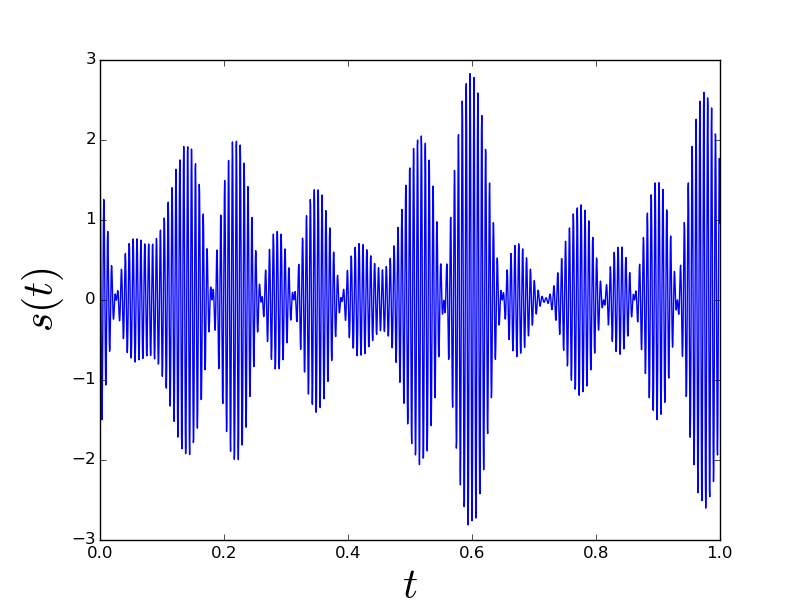
\includegraphics[width=\textwidth]{domain/am_example_time}
    \caption{}
  \end{subfigure}
  \begin{subfigure}{0.45\textwidth}
    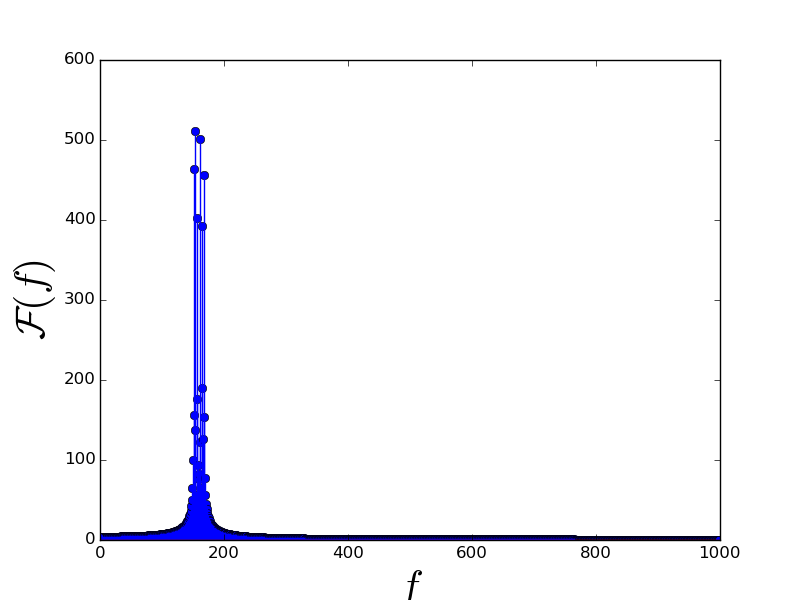
\includegraphics[width=\textwidth]{domain/am_example_freq}
    \caption{}
  \end{subfigure}
  \caption{Временная (а) и частотная (б) диаграммы амплитудно модулированного сигнала}
  \label{fig:domain:am}
\end{figure}

\subsubsection{Фазовая модуляция (PM).}\ Модулирующий сигнал воздействует на полную фазу несущей. Лишена недостатков AM, но на практике применяются только ее модификации. Временная диаграмма показывает, что мгновенная частота модулированного сигнала прямо пропорциональна производной по времени исходного. Так удобно, например, кодировать дискретные сигналы с высокой устойчивостью к аддитивным помехам. Однако, модулированный сигнал передает только изменение исходного, но не его самого. Если кодируется двоичная информация, то пропуск одного перехода повлечет инверсию все последующих бит. Формула PM приведена ниже (\autoref{eq:domain:pm}).

\begin{equation}
  \label{eq:domain:pm}
  s(t) = A_0 cos(\omega_0 t + m s(t))
\end{equation}
\begin{explanation}
\item[где] $A_0$ --- амплитуда несущей.
\item $\omega_0$ --- частота несущей.
\item $m$ --- девиация фазы.
\item $s_m(t)$ --- модулирующий сигнал.
\end{explanation}

\begin{figure}[h]
  \centering
  \begin{subfigure}{0.45\textwidth}
    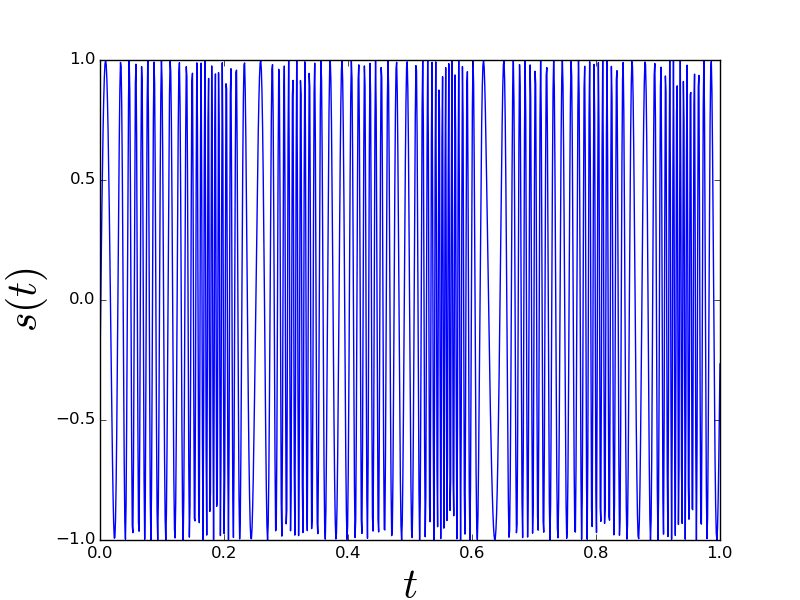
\includegraphics[width=\textwidth]{domain/pm_example_time}
    \caption{}
  \end{subfigure}
  \begin{subfigure}{0.45\textwidth}
    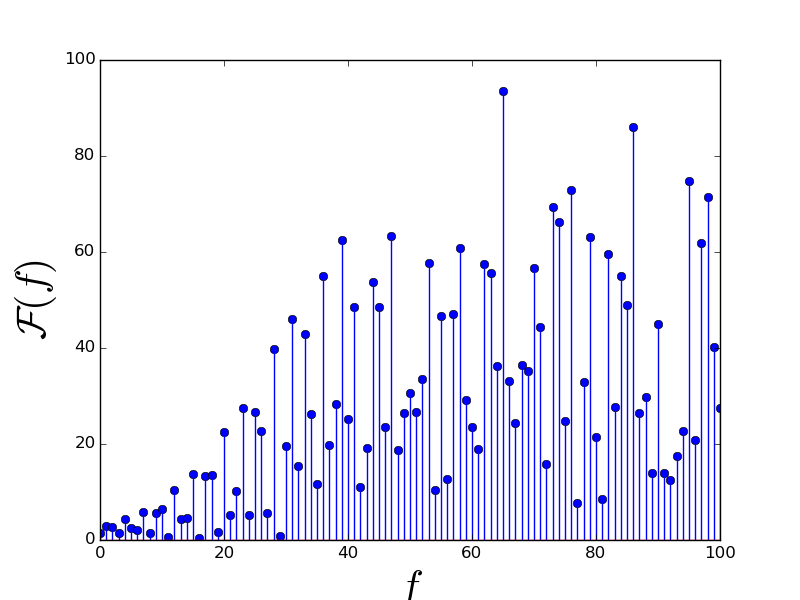
\includegraphics[width=\textwidth]{domain/pm_example_freq}
    \caption{}
  \end{subfigure}
  \caption{Временная (а) и частотная (б) диаграммы фазово модулированного сигнала}
  \label{fig:domain:pm}
\end{figure}


\subsubsection{Частотная модуляция (FM).}\ Модулирующий сигнал воздействует на мгновенную частоту несущей. Самый распространенный и известный тип модуляции. FM приобрела популярность из-за высокой помехоустойчивости (как и PM), высокого КПД передачи и эффективности использования выделенной полосы частот. Узкополосный режим позволяет разместить большое число передатчиков в ограниченном диапазоне частот (используется для служебной связи), а широкополосный --- значительно увеличить отношение мощности сигнала к шуму (используется в коммерческом радиовещании). Ниже приведено выражение для частотной модуляции (\autoref{eq:domain:fm}).

\begin{equation}
  \label{eq:domain:fm}
  s(t) = A_0 cos(\omega_0 t + \omega_d \int{s_m(t)dt}  + \phi_0)
\end{equation}
\begin{explanation}
\item[где] $A_0$ --- амплитуда несущей.
\item $\omega_0$ --- частота несущей.
\item $\omega_d$ --- девиация частоты.
\item $s_m(t)$ --- модулирующий сигнал.
\item $\phi_0$ --- начальная фаза несущей.
\end{explanation}

\begin{figure}[h]
  \centering
  \begin{subfigure}{0.45\textwidth}
    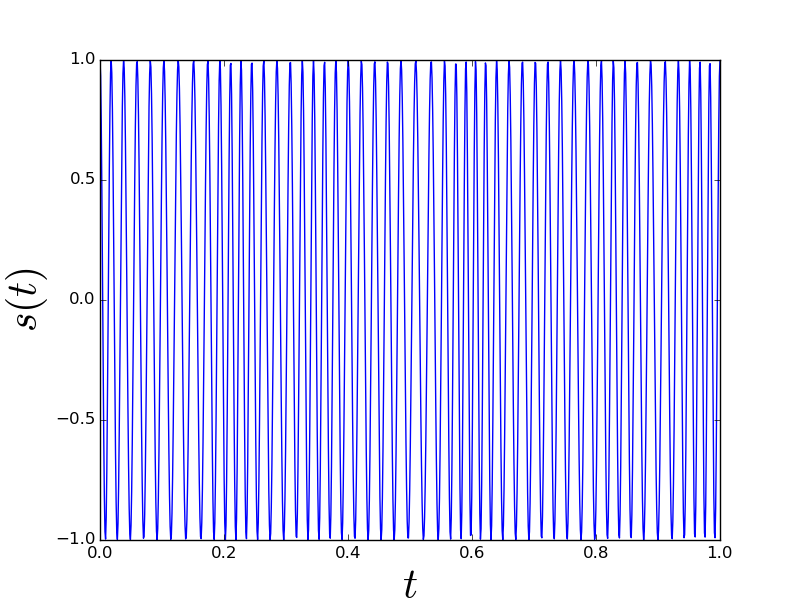
\includegraphics[width=\textwidth]{domain/fm_example_time}
    \caption{}
  \end{subfigure}
  \begin{subfigure}{0.45\textwidth}
    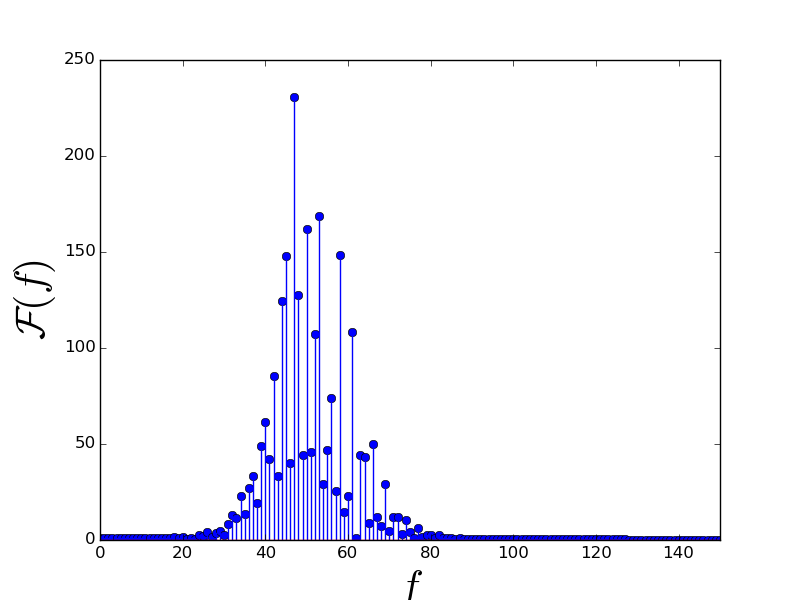
\includegraphics[width=\textwidth]{domain/fm_example_freq}
    \caption{}
  \end{subfigure}
  \caption{Временная (а) и частотная (б) диаграммы частотно модулированного сигнала}
  \label{fig:domain:fm}
\end{figure}

Рассмотренные выше методы являются фундаментальными --- они определяют три ключевых направления модуляции несущего сигнала. От них было порождено множество производных, устраняющих те или иные недостатки родителя.

Стоит упомянуть отдельно семейство методов, где модулирующим является дискретный сигнал. Цифровая модуляция даже получила отдельное название --- манипуляция. Она находит все большее применение в служебной и коммерческой связи из-за своей эффективности, помехоустойчивости и способности передавать цифровой сигнал без предварительного преобразования в аналоговую форму (это делается при модуляции). В данный момент на цифровую связь переведена большая часть служебных передач в городе Минске, а Норвегия объявила о намерении полностью заместить FM вещание на DAB и DAB+ \cite{norway_dab}.

Переход к новому способу связи это очень серьезное решение, так как старое оборудование не способно работать с новыми типами модуляции. Имеющиеся передатчики и приемники становятся совершенно бесполезными. Более того, страна, перешедшая на цифровой формат коммерческого вещания оказывается изолированной от передач соседей, если те работают в аналоге. Но какими бы страшными не казались проблемы миграции, технологический и как следствие экономический эффект в перспективе превышают расходы.

\subsection{Типы помех (2)}

В общем виде реальный сигнал можно рассматривать как совокупность передаваемого сигнала и воздействующих на него помех (\autoref{eq:domain:noise_types}).

\begin{equation}
  \label{eq:domain:noise_types}
  s(t) = k(t) e(t) + n(t)
\end{equation}
\begin{explanation}
\item[где] $e(t)$ --- передаваемый сигнал.
\item $k(t)$ --- коэффициент мультипликативной помехи.
\item $n(t)$ --- коэффициент аддитивной помехи.
\end{explanation}

Мультипликативные помехи возникают по причине изменения характеристик среды передачи с течением времени. Это может быть нагрев элементов радиосистемы, воздействие атмосферных явлений и др. Как правило, они действуют в течении длительного временного интервала и не мешают мгновенному приему и распознанию сигнала, поэтому опустим их подробное рассмотрение и сконцентрируемся на аддитивных помехах.

Аддитивные помехи представляют собой независимые добавки к принимаемому сигналу. Их разнообразие очень велико --- от реликтового излучения до преднамеренного зашумления эфира. Именно они могут оказывать существенное влияние на качество приема, поэтому стоит ознакомиться с их классификацией.

\subsubsection{По закону распределения}\ их разделяют на гауссовские и негауссовские. Такое деление удобно из-за того, что большая часть естественных помех подчиняется нормальному закону распределения. Это объясняется центральной предельной теоремой --- характер распределения суммы множества слабо взаимосвязанных помех, где ни одна не доминирует над остальными сходится к нормальному. Более того, часто можно принимать их математическое ожидание равным нулю. Негауссовские помехи учитывать сложнее, но обычно их тоже можно описывать случайным процессом с известным законом распределения.

\subsubsection{По характеру стационарности}\ выделяют стационарные и нестационарные помехи. Как и в теории случайных процессов, первые не изменяют характеристик своего распределения во времени, а вторые изменяют. В целях обнаружения сигнала часто предполагают, что помеха описывается стационарным случайным процессом с гауссовским законом распределения. Их также называют флуктуационные.

\subsubsection{По механизму возникновения}\ помехи разделяются на естественные, индустриальные, системные и искусственные.

Естественными помехами могут быть шумы в радиоприемном тракте, а также космические и атмосферные влияния. До нас непрерывно доходит шум Метагалактики, на фон которого накладываются излучения планет и звезд. Грозовая деятельность порождает еще один источник нежелательной активности в радиоэфире.

Индустриальные помехи создаются электрическими и электронными устройствами. Зачастую они носят импульсный характер: короткие всплески со сравнительно длительными периодами бездействия.

Системные помехи создаются другими радиотехническими средствами. Они также называются сосредоточенными, так как расположены в узком частотном интервале. Их могут вызвать близко расположенные радиостанции или большое число удаленных. Мешающее воздействие не обязательно объясняется перекрывающимися интервалами частот --- его причиной может быть отражение и рассеяние сигналов в атмосфере. Задача обеспечения электромагнитной совместимости сложна и пути ее решения описаны в отдельных научных работах.

Искусственные помехи создаются с целью мешающего действия радиосредствам. Использование таких форм помех в процессе военных действий является одной из форм "радиоэлектронной войны". Их формы очень разнообразны, но основная задача одна --- создание помехового фона, затрудняющего прием полезного сигнала или имитирование ложных целей.
\\

В целях дипломного проекта необходимо в первую очередь учитывать естественные флуктуационные помехи. Они всегда присутствуют в реальных условиях приема и могут быть описаны несложными математическими моделями. Иные типы помех встречаются достаточно редко и требуют специфических методов обработки.

\subsection{Комплексное представление сигнала (2)}
\subsection{Временной и частотный анализ (3)}


\section{Аппаратное обеспечение}
\label{sec:hardware}


\subsection{\SDR-приемник}

\sdr\ (\SDR) --- это разновидность радиосистем, в которых компоненты, традиционно реализуемые аппаратно, замещены программными модулями.
В идеале, из аналоговых устройств хотелось бы оставить только антенну и подключенный к ней аналого-цифровой преобразователь. Все остальные манипуляции с сигналом осуществлялись бы программно. Эта схема обеспечила бы максимальную гибкость и универсальность. Большую часть приемо-передающего тракта можно было бы модифицировать простым обновлением прошивки устройства.
Однако, в настоящее время удовлетворительная частота и точность работы ЦАП и АЦП может быть достигнута только с помощью физических эффектов, таких как интерференция и резонанс. Чтобы привести сигнал к промежуточной частоте используется супергетеродинный приемник. Эти требования увеличивают аналоговую прослойку между антенной и программным обеспечением, но она универсальна и не накладывает концептуальных ограничений на типы принимаемых сигналов.

\begin{figure}[h]
  \centering
  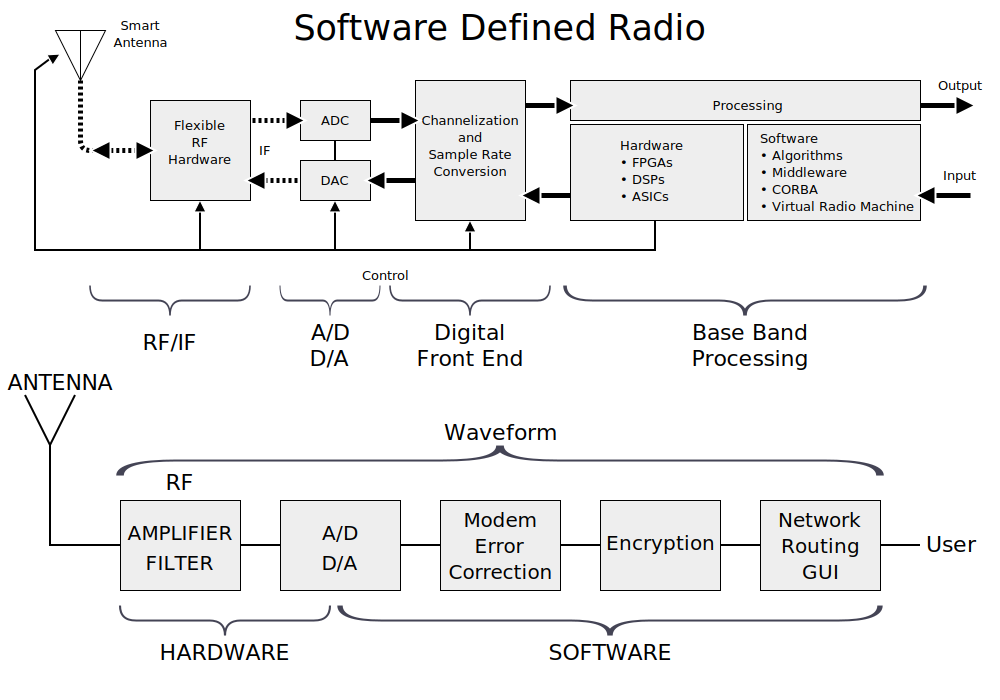
\includegraphics[width=0.8\textwidth]{hardware/sdr_pipeline}
  \caption{Схема работы приемно-передающего тракта \SDR\ \cite{sdr_wiki}}
  \label{fig:hardware:sdr_pipeline}
\end{figure}

Идея \SDR\ не нова --- разработки ведутся с конца \Romannum{20} века. Тогда они не были доступны широкой публике, а программные компоненты создавались для конкретной компьютерной архитектуры. Данные факторы ограничивали развитие этой области радиотехники в основном военными целями.

Положение дел изменилось в 2010 году, когда радиолюбители обнаружили, что ТВ-тюнер Realtek 2832U осуществляет обработку принимаемого сигнала программно. Спецификация платы и протокол взаимодействия ее компонент не были доступны публично, поэтому в следующие годы любители занимались его реверс-инжинирингом. Итогом их действий стала плата на основе вышеупомянутого ТВ-тюнера, способная принимать сигнал с антенны и передавать его комплексное представление приложениям через USB порт.

Стоимость такого устройства невелика --- от \$10 до \$20. Для сравнения, традиционные радиосредства, обладающие сравнимыми характеристиками стоили от \$300 и выше, при том что они поддерживали только несколько протоколов связи. Этот факт дал начало масштабному проникновению \SDR\ в круг энтузиастов. В последние годы это направление бурно развивается, появляются как прикладные приложения, так и аппаратные средства с усовершенствованными характеристиками. В дипломном проекте использовался модифицированный DVB-T тюнер R820T2 (\autoref{fig:hardware:rtl_sdr}).

\begin{figure}[h]
  \centering
  \begin{subfigure}{0.45\textwidth}
    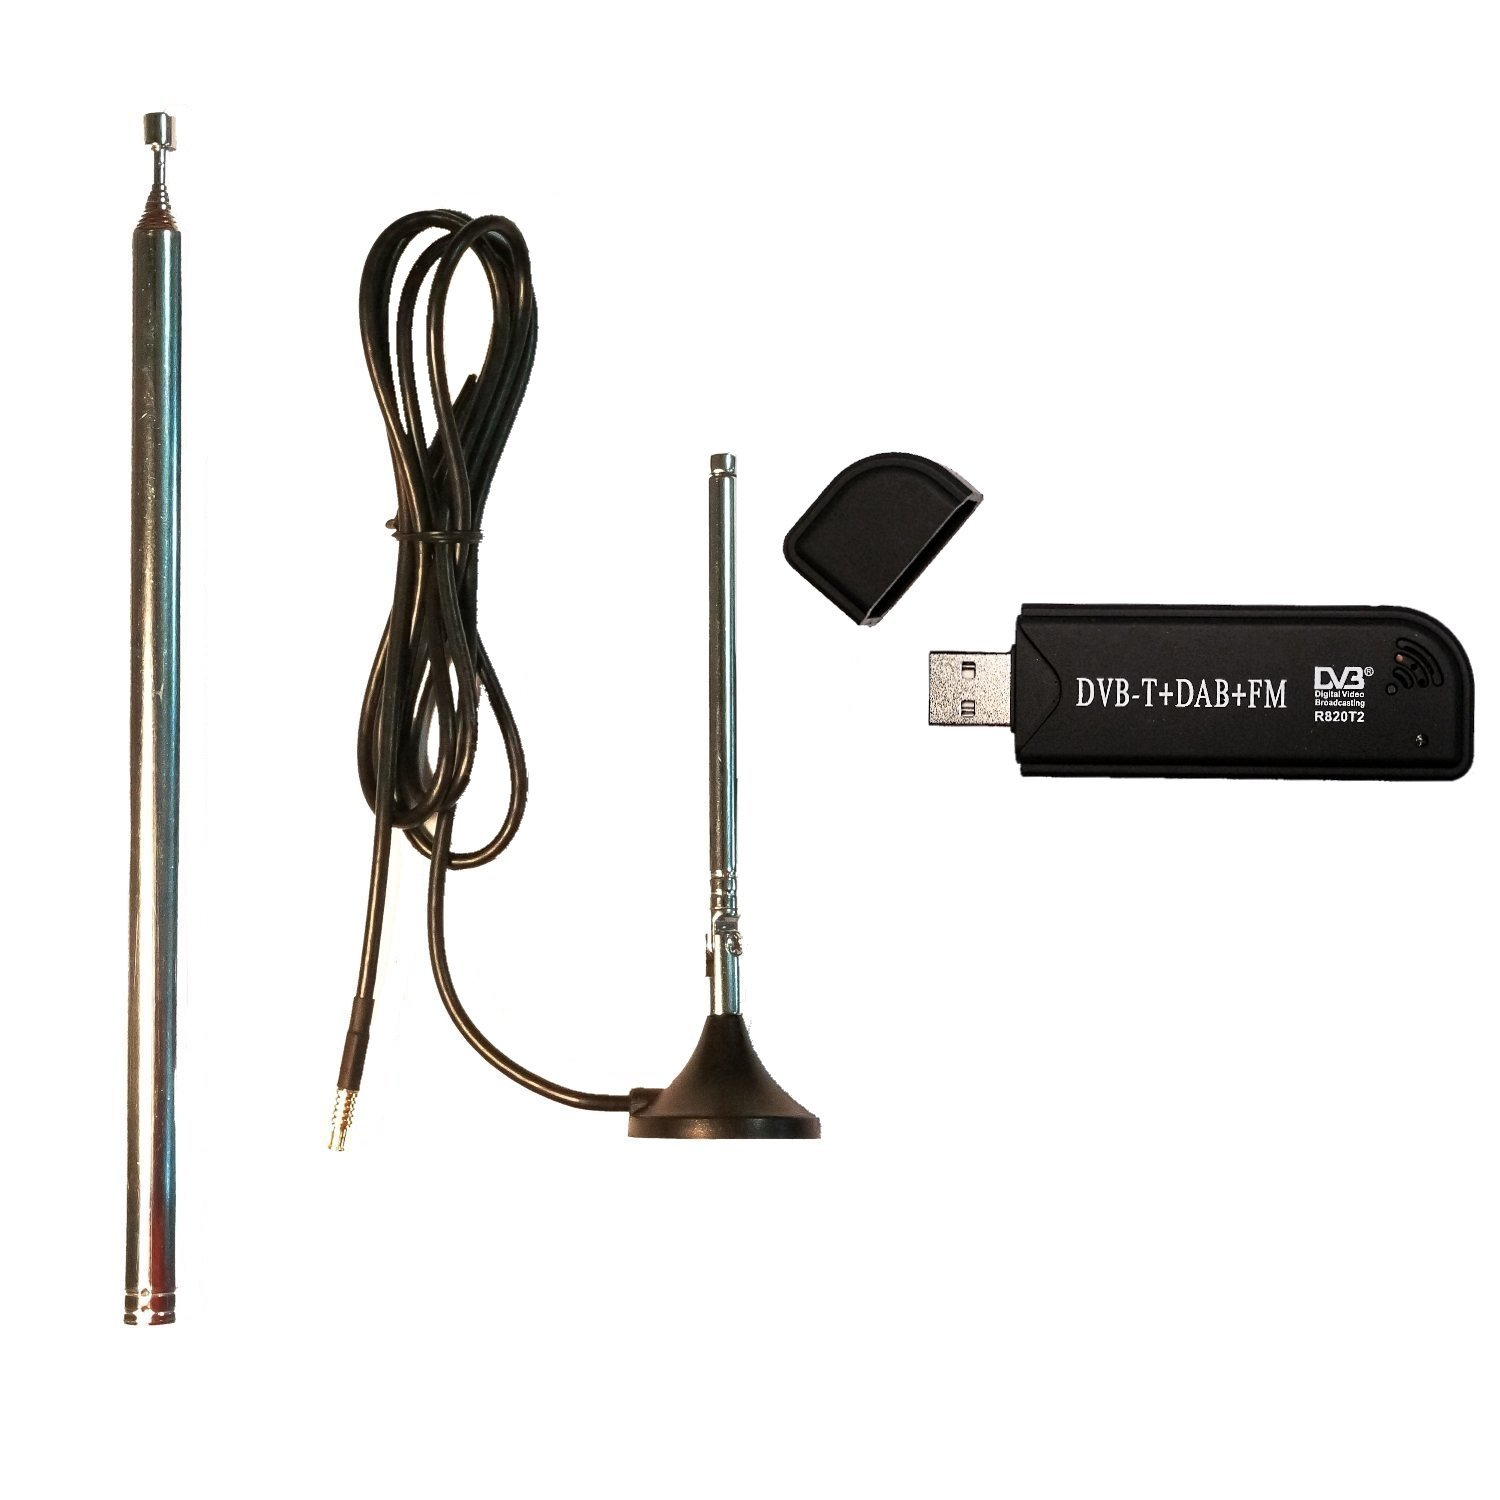
\includegraphics[width=\textwidth]{hardware/rtl_sdr_set}
    \caption{}
    \label{fig:hardware:rtl_sdr_set}
  \end{subfigure}
  \begin{subfigure}{0.45\textwidth}
    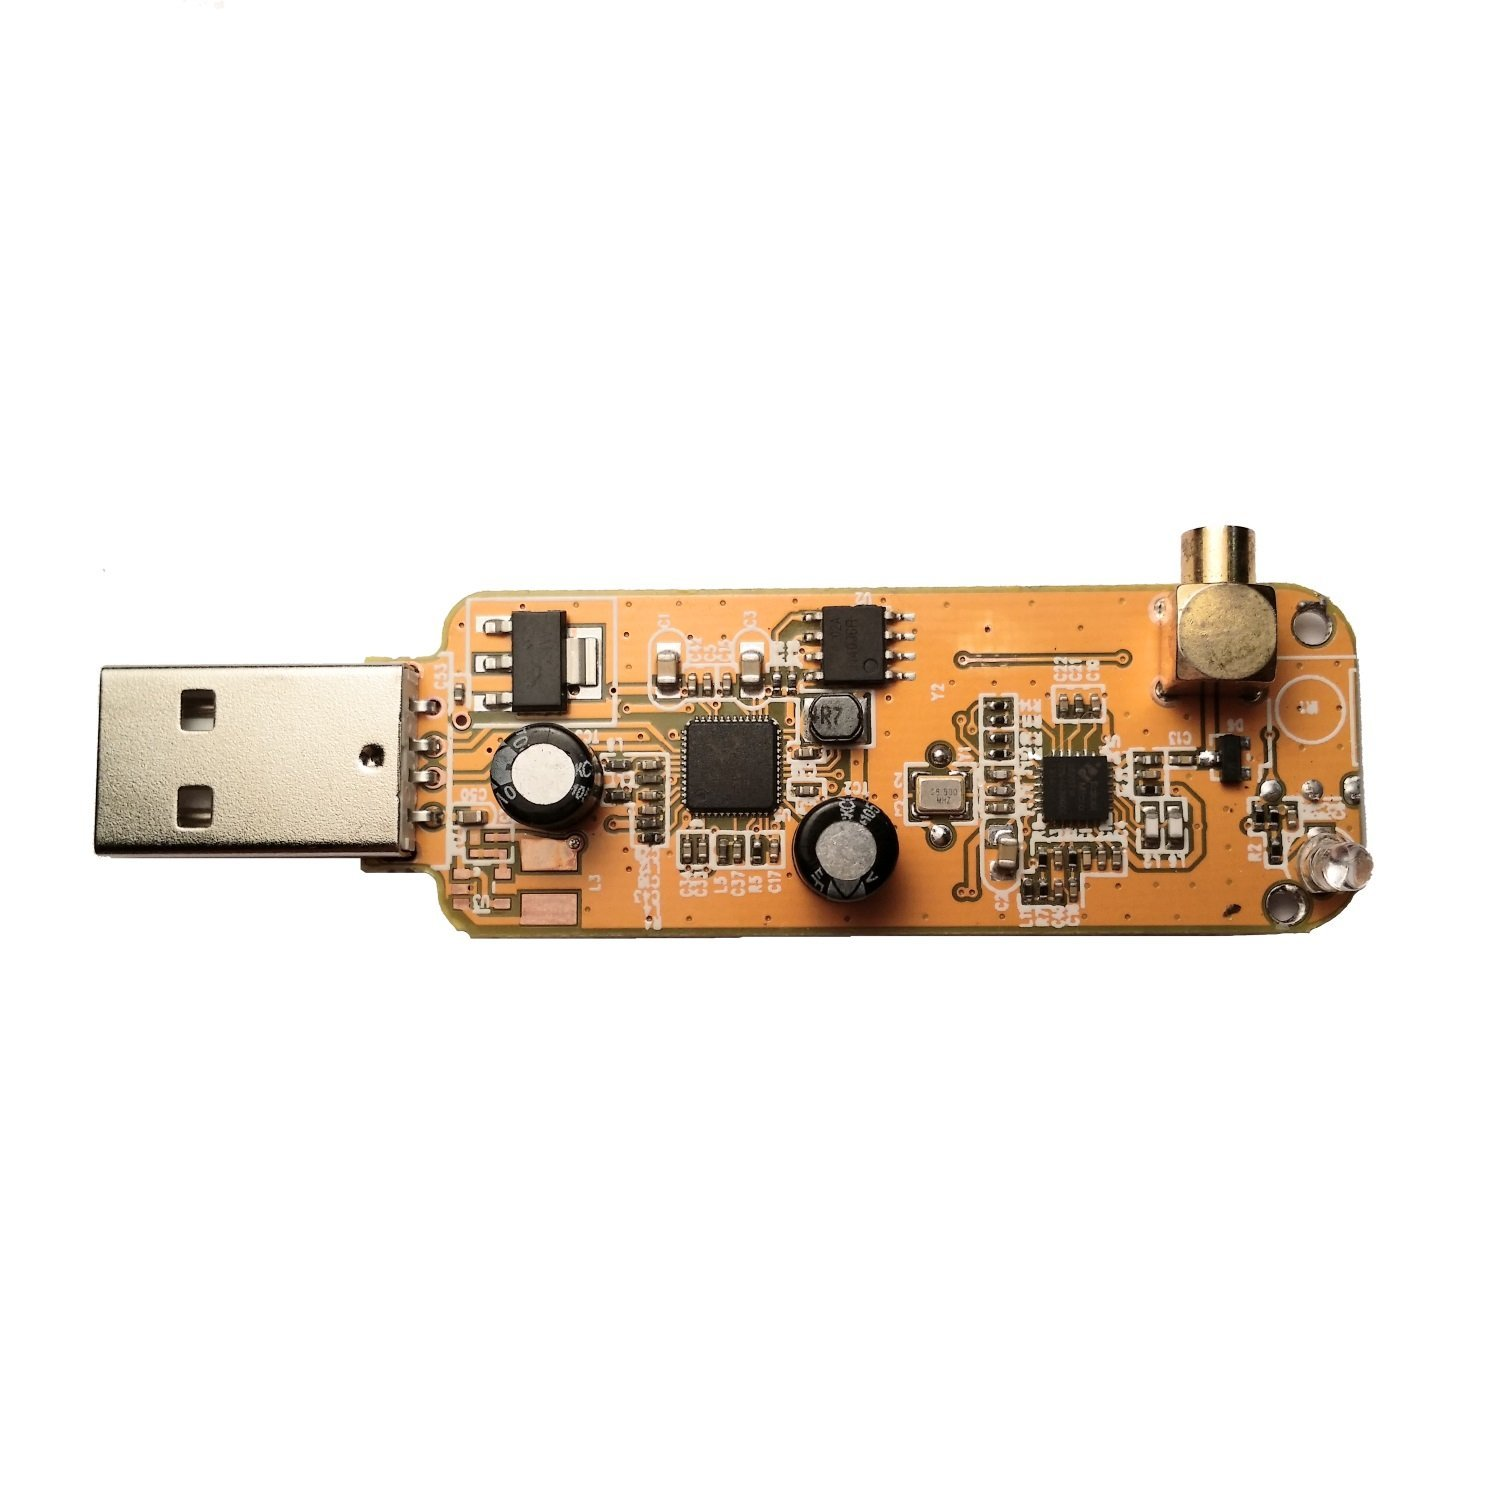
\includegraphics[width=\textwidth]{hardware/rtl_sdr_stripped}
    \caption{}
    \label{fig:hardware:rtl_sdr_stripped}
  \end{subfigure}
  \caption{Готовый к использованию комплект \sdr\ (\subref{fig:hardware:rtl_sdr_set}), внешний вид тюнера без пластикового корпуса (\subref{fig:hardware:rtl_sdr_stripped})}
  \label{fig:hardware:rtl_sdr}
\end{figure}

Определяющим фактором эффективности \SDR\ являются параметры ЦАП и АЦП. Они задают максимальную ширину рабочей полосы частот. В используемом устройстве она ограничена примерно двумя мегагерцами. Это не позволяет использовать его, например, для полноценного приема спутникового телевидения, полоса частот которого шире \SI{2}{\mega\hertz}. В них помещается только звук и черно-белое изображение. Теоретически, можно использовать несколько синхронизированных приемников для увеличения общей ширины полосы, но на практике из-за сложности синхронизации обычно производят замену преобразователей на более мощные.

\subsection{Антенна}

Выбор антенны очень важен для достижения наилучшего качества и дальности передачи. Но мне нужен только прием, поэтому задача значительно упрощается.
В комплект поставки \SDR\ входили две телескопических штыревых антенны длиной до \SI{31.5}{см} и \SI{1.5}{м}. Для исследовательских целей их оказалось достаточно.

Длина антенны прямо пропорциональна максимальной длине волны, которую можно на нее принять. Полтора метра хватает на заявленный диапазон работы Realtek R820T2 --- от \SI{24}{\mega\hertz} до \SI{1.7}{\giga\hertz}.

Достаточно большая полоса частот ниже меньшей границы не может быть использована со стандартными средствами. Но их можно заменять и радиолюбители предлагают использовать в качестве антенны для длинных волн кусок кабеля, вывешенный за окно. Качество приема будет не идеальным, но он закроет неприятную "дыру" ниже \SI{24}{\mega\hertz} в рабочем спектре.

Верхняя граница обусловлена характеристиками преобразователя к промежуточной частоте --- целевое использование устройства было ТВ-тюнером, поэтому оно просто не было спроектировано для работы вне своего диапазона. Сейчас на рынке имеется большое число "чистокровных" \SDR\ со значительно лучшими техническими характеристиками.


\subsection{Субдискретизация}

Как было упомянуто, верхняя граница рабочего диапазона частот находится немногим ниже двух гигагерц, при том что частота дискретизации устройства всего-лишь \SI{2.6}{\mega\sample\per\second} (\num{2.6} миллиона семплов в секунду). Из теоремы Котельникова (Найквиста-Шеннона) следует, что восстановить аналоговый сигнал по дискретной выборке его моментальных значений (семплов) можно только тогда, когда частота дискретизации превышает максимальную частоту компонент сигнала не менее чем в два раза. Следовательно, при частоте дискретизации равной \SI{2.6}{\mega\sample\per\second} получилось бы оцифровать сигнал частотой не более \SI{1.3}{\mega\hertz}. Это так для реальных семплов и сигнала, лежащего в основной полосе частот, но в нашем случае инженерные приемы позволяют работать с этим ограничением.

Во первых, обычно нас интересует не весь диапазон частот от нуля до максимальной, а только определенная полоса, например, \SI{50}{\kilo\hertz} в случае узкополосной FM связи. Если бы она начиналась с нулевой частоты, то никаких технических проблем бы не возникло, но FM диапазон находится как правило выше семидесяти мегагерц и напрямую достать до этой полосы не получается.

В этом случае используется переход к промежуточной частоте. Этот метод основывается на том, что при смешивании двух сигналов с частотами $f_0$ и $f_1$ возникают сигналы с частотами $f_0 - f_1$ и $f_0 + f_1$. Таким образом, можно смешать целевой и близкий к нему сигналы, чтобы "сместить" интересующую нас полосу к нулевой частоте, а затем применить полосовой фильтр, для удаления лишней информации. Конечно, точные значения исходного сигнала теряются, но его по-прежнему можно демодулировать и извлечь полезные данные --- промежуточная частота сохраняет амплитуду и относительную мгновенную частоту.

Во вторых, \SDR\ представляет сигнал в комплексной форме, из-за чего минимальная частота, требуемая теоремой Котельникова, уменьшается вдвое. Комплексный сигнал более "насыщен" информацией. Отрицательные частоты в нем не дублируют положительные. Правда, для получения одного значения нужно иметь два реальных. Поэтому при сравнении АЦП, работающих с комплексным и реальным представлением, можно сказать, что у первых эффективная частота дискретизации в два раза выше номинальной.

Но даже применение этих методов не спасает от ограничения рабочего диапазона частот, который определяется характеристиками гетеродина. Чтобы поднять этот потолок нужно генерировать стабильные колебания на очень высоких частотах. Бюджетные устройства пока не могут позволить себе элементов такого качества.


\subsection{Сравнительный анализ аппаратных средств}

Когда программное радио начало набирать популярность у хоббистов, на рынке стали стремительно появляться новые модели устройств с самыми разными характеристиками и ценами. Сейчас выбор варьируется от модифицированного ТВ-тюнера до профессиональных плат, способных принимать и передавать даже Wi-Fi сигнал.

Hi-end платы уже не просто приемники и передатчики. Они содержат FPGA, который можно использовать для выхода за рамки эффективности компьютера общего назначения. FPGA --- это разновидность ПЛИС, особенностью которой является изменение конфигурации соединений по сигналу, посылаемогу плате. Гибкость соединений и эффективность в работе с блоками данных обеспечили им широкое распространение в области цифровой обработки сигналов, поэтому многие \SDR имеют этот элемент в своей конструкции.

Также популярным оказалось решение использовать несколько параллельно работающих АЦП, чтобы охватить больший участок спектра. Например, в модели Crimson их четыре, за счет чего принимаемая полоса частот на порядок выше многих конкурентов --- \SI{800}{\mega\hertz}.

Некоторые образцы имеют даже веб интерфейс с возможностью удаленного управления.

Ниже приведено сравнение основных характеристик наиболее ярких представителей различных ценовых диапазонов (\autoref{table:hardware:boards}).


\begingroup
\renewcommand{\arraystretch}{1.5}
\begin{table}[h]
  \centering
  \begin{tabular}{|>{\centering}m{0.2\textwidth}
                  |>{\centering}m{0.1\textwidth}
                  |>{\centering}m{0.1\textwidth}
                  |>{\centering}m{0.1\textwidth}
                  |>{\centering}m{0.1\textwidth}
                  |>{\centering}m{0.1\textwidth}
                  |>{\centering\arraybackslash}m{0.1\textwidth}|}
    \hline
    & Realtek 2832U & HackRF & bladeRF & USRP B200 & UmTRX & Crimson \\
    \hline
    Минимальная рабочая частота, \si{\mega\hertz} & \num{24} & \num{30} & \num{300} & \num{50} & \num{300} & \num{0.1} \\
    \hline
    Максимальная рабочая частота, \si{\mega\hertz} & \num{1700} & \num{6000} & \num{3800} & \num{6000} & \num{3800} & \num{6000} \\
    \hline
    Частота дискретизации, \si{\mega\hertz} & \num{3.2} & \num{20} & \num{28} & \num{61.44} & \num{40} & \num{800} \\
    \hline
    Разрядность, \si{\bit} & \num{8} & \num{8} & \num{12} & \num{12} & \num{12} & \num{16} \\
    \hline
    Передатчик & - & + & + & + & + & + \\
    \hline
    Стоимость, \$ & \num{20} & \num{300} & \num{420} & \num{675} & \num{950} & \num{6500} \\
    \hline
  \end{tabular}
  \caption{Характеристики некоторых моделей \SDR}
  \label{table:hardware:boards}
\end{table}
\endgroup


%\include{sections/tech}

%\include{sections/arch_and_mod}

%\newcommand{\yandex}{ООО \mbox{<<Яндекс>>}}
\newcommand{\yandexbel}{ООО \mbox{<<ЯндексБел>>}}
\newcommand{\rubinplaza}{\mbox{<<Рубин Плаза>>}}

\section{Охрана труда}

\subsection[Обеспечение пожарной безопасности на предприятии]{Обеспечение пожарной безопасности на предприятии \yandexbel{}}

Целью дипломного проектирования явилась разработка программного средства для обнаружения радиосигналов с помощью SDR-приемника. С его помощью можно сканировать радиоэфир, выделяя наиболее сильные источники сигнала, а также исследовать отдельные частоты, определяя нешумовые последовательности. Аппаратная часть проекта обеспечена приемником на базе software defined radio, что позволяет значительно сократить материальные расходы в сравнении с традиционными системами. В настоящем разделе рассмотрим вопросы, связанные с обеспечением пожарной безопасности в компании \yandexbel{}.

Разработка выполнялась при прохождении преддипломной практики в компании \yandexbel{}. \yandexbel{} --- дочерняя компания \yandex{}. Основным направлением ее деятельности является разработка программного обеспечения. Белорусскому офису всего несколько лет, но сейчас там работает более ста человек и ожидается дальнейший рост. Офис располагается в двух блоках бизнес-центра \rubinplaza{}.

\rubinplaza --- современный бизнес-центр категории Б. Помимо \yandexbel{} в нем работают команды EPAM Systems, Onliner, БПС-Сбербанк. Планировка здания обеспечивает высокий уровень пожарной безопасности. Каждый офисный блок имеет два выхода. Парадный выход оборудован лифтами и лестницей, пожарный --- только лестницей. На каждом этаже имеется свободный доступ к им обоим. Огнезащитное покрытие конструкций изолирует секции этажа, предотвращая распространение пламени.

Въезд на территорию бизнес-центра контроллируеся охраной. Блокирование проездов и проходов не допускается. Внешняя сторона здания остеклена, что позволяет использовать оконные проемы для экстренного доступа в помещения.

Для отопления помещений используются приборы центрального водяного отопления. Воздухонагревательные приборы объединены в вентиляционную систему здания. Воздуховоды вмонтированы в межэтажные перекрытия и недоступны извне. Электросеть здания также проложена в межсекционных перегородках и межэтажных перекрытиях. Для подключения к ней в стены встроены розетки. Работники компании подключаются к электросети через сетевые фильры, защищающие от резких скачков напряжения. В помещениях имеется достаточное количество розеток для подключения всего необходимого электрооборудования сотрудников.

За пожарную безопасность в \yandexbel{} отвечает директор компании. После найма сотрудники проходят инструктаж по установленному противопожарному режиму и мерам безопасности при работе с электрооборудованием. Курение внутри здания запрещено, в каждом помещении установлены пожарные извещатели. Рабочие места организованы таким образом, чтобы организовать беспрепятственный доступ к сетевым фильтрам и проложить кабели электроприборов вне рабочей области людей.

В коридорах установлены пожарные краны (рисунок \ref{fig:fireplug}). Ключи к ним находятся в специальных застекленных отсеках и в случае экстренной ситуации могут быть быстро извлечены без посторонней помощи. Пожарные краны сгруппированы в блоки примерно по 2 крана на кабинет. Для оперативного тушения пламени в кабинетах установлены порошковые огнетушители (рисунок \ref{fig:extinguisher}) и оросительная система пожаротушения.

Каждый кабинет оборудован пожарным дымовым оптико-электрическим точечным извещателем \mbox{ИП212-02М1} (рисунок \ref{fig:auto_fire_detector}). В коридорах дополнительно установлены ручные пожарные извещатели \mbox{ИП 5-2Р} (рисунок \ref{fig:manual_fire_detector}).

Таким образом, изложенные выше предложения обеспечивают пожарную безопасность в компании \yandexbel{}.

\begin{figure}
  \begin{center}
    
\includegraphics[height=0.4\textheight]{auto_fire_detector}
    \caption{Автономный пожарный извещатель}
    \label{fig:auto_fire_detector}

    \vspace{0.05\textheight}

    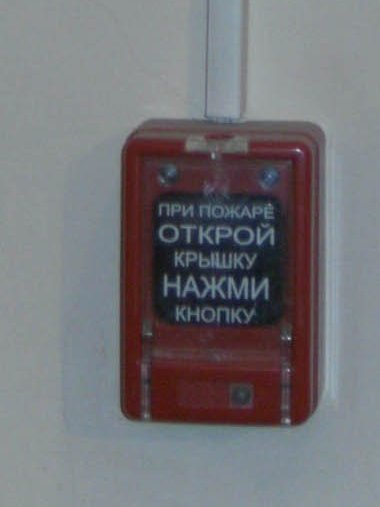
\includegraphics[height=0.4\textheight]{manual_fire_detector}
    \caption{Ручной пожарный извещатель}
    \label{fig:manual_fire_detector}
  \end{center}
\end{figure}

\begin{figure}
  \begin{center}
    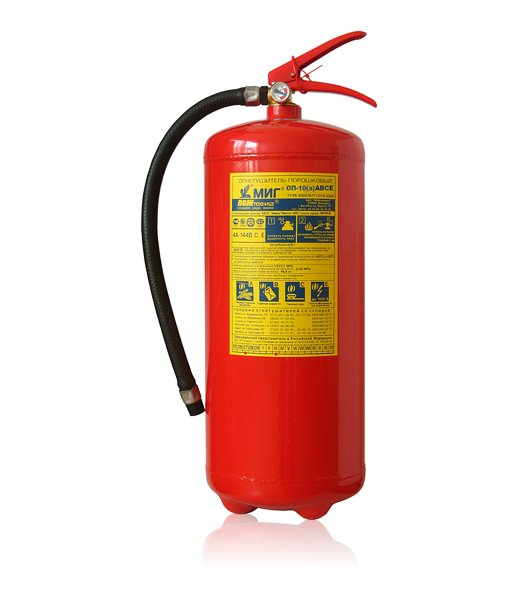
\includegraphics[height=0.4\textheight]{extinguisher}
    \caption{Порошковый огнетушитель \mbox{ОП-10} (з) МИГ М}
    \label{fig:extinguisher}

    \vspace{0.05\textheight}

    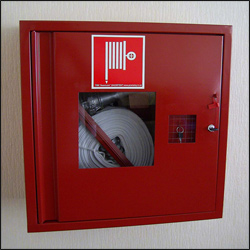
\includegraphics[height=0.4\textheight]{fireplug}
    \caption{Пожарный кран}
    \label{fig:fireplug}
  \end{center}
\end{figure}

%\newcommand{\byr}{Br}

\section{Технико-экономическое обоснование}

% Begin Calculations

\FPeval{\totalProgramSize}{15680}
\FPeval{\totalProgramSizeCorrected}{8650}

\FPeval{\normativeManDays}{224}

\FPeval{\additionalComplexity}{0.12}
\FPeval{\complexityFactor}{clip(1 + \additionalComplexity)}

\FPeval{\stdModuleUsageFactor}{0.7}
\FPeval{\originalityFactor}{0.7}

\FPeval{\adjustedManDaysExact}{clip( \normativeManDays * \complexityFactor * \stdModuleUsageFactor * \originalityFactor )}
\FPround{\adjustedManDays}{\adjustedManDaysExact}{0}

\FPeval{\daysInYear}{365}
\FPeval{\redLettersDaysInYear}{9}
\FPeval{\weekendDaysInYear}{104}
\FPeval{\vocationDaysInYear}{21}
\FPeval{\workingDaysInYear}{ clip( \daysInYear - \redLettersDaysInYear - \weekendDaysInYear - \vocationDaysInYear ) }

\FPeval{\developmentTimeMonths}{3}
\FPeval{\developmentTimeYearsExact}{clip(\developmentTimeMonths / 12)}
\FPround{\developmentTimeYears}{\developmentTimeYearsExact}{2}
\FPeval{\requiredNumberOfProgrammersExact}{ clip( \adjustedManDays / (\developmentTimeYears * \workingDaysInYear) + 0.5 ) }

% тут должно получаться 2 ))
\FPtrunc{\requiredNumberOfProgrammers}{\requiredNumberOfProgrammersExact}{0}

\FPeval{\tariffRateFirst}{600000}
\FPeval{\tariffFactorFst}{3.04}
\FPeval{\tariffFactorSnd}{3.48}


\FPeval{\employmentFstExact}{clip( \adjustedManDays / \requiredNumberOfProgrammers )}
\FPtrunc{\employmentFst}{\employmentFstExact}{0}

\FPeval{\employmentSnd}{clip(\adjustedManDays - \employmentFst)}


\FPeval{\workingHoursInMonth}{160}
\FPeval{\salaryPerHourFstExact}{clip( \tariffRateFirst * \tariffFactorFst / \workingHoursInMonth )}
\FPeval{\salaryPerHourSndExact}{clip( \tariffRateFirst * \tariffFactorSnd / \workingHoursInMonth )}
\FPround{\salaryPerHourFst}{\salaryPerHourFstExact}{0}
\FPround{\salaryPerHourSnd}{\salaryPerHourSndExact}{0}

\FPeval{\bonusRate}{1.5}
\FPeval{\workingHoursInDay}{8}
\FPeval{\totalSalaryExact}{clip( \workingHoursInDay * \bonusRate * ( \salaryPerHourFst * \employmentFst + \salaryPerHourSnd * \employmentSnd ) )}
\FPround{\totalSalary}{\totalSalaryExact}{0}

\FPeval{\additionalSalaryNormative}{20}

\FPeval{\additionalSalaryExact}{clip( \totalSalary * \additionalSalaryNormative / 100 )}
\FPround{\additionalSalary}{\additionalSalaryExact}{0}

\FPeval{\socialNeedsNormative}{0.5}
\FPeval{\socialProtectionNormative}{34}
\FPeval{\socialProtectionFund}{ clip(\socialNeedsNormative + \socialProtectionNormative) }

\FPeval{\socialProtectionCostExact}{clip( (\totalSalary + \additionalSalary) * \socialProtectionFund / 100 )}
\FPround{\socialProtectionCost}{\socialProtectionCostExact}{0}

\FPeval{\taxWorkProtNormative}{4}
\FPeval{\taxWorkProtCostExact}{clip( (\totalSalary + \additionalSalary) * \taxWorkProtNormative / 100 )}
\FPround{\taxWorkProtCost}{\taxWorkProtCostExact}{0}
\FPeval{\taxWorkProtCost}{0} % это считать не нужно, зануляем чтобы не менять формулы

\FPeval{\stuffNormative}{3}
\FPeval{\stuffCostExact}{clip( \totalSalary * \stuffNormative / 100 )}
\FPeval{\stuffCost}{\stuffCostExact}

\FPeval{\timeToDebugCodeNormative}{15}
\FPeval{\reducingTimeToDebugFactor}{0.3}
\FPeval{\adjustedTimeToDebugCodeNormative}{ clip( \timeToDebugCodeNormative * \reducingTimeToDebugFactor ) }

\FPeval{\oneHourMachineTimeCost}{5000}

\FPeval{\machineTimeCostExact}{ clip( \oneHourMachineTimeCost * \totalProgramSizeCorrected / 100 * \adjustedTimeToDebugCodeNormative ) }
\FPround{\machineTimeCost}{\machineTimeCostExact}{0}

\FPeval{\businessTripNormative}{15}
\FPeval{\businessTripCostExact}{ clip( \totalSalary * \businessTripNormative / 100 ) }
\FPround{\businessTripCost}{\businessTripCostExact}{0}

\FPeval{\otherCostNormative}{20}
\FPeval{\otherCostExact}{clip( \totalSalary * \otherCostNormative / 100 )}
\FPround{\otherCost}{\otherCostExact}{0}

\FPeval{\overheadCostNormative}{100}
\FPeval{\overallCostExact}{clip( \totalSalary * \overheadCostNormative / 100 )}
\FPround{\overheadCost}{\overallCostExact}{0}

\FPeval{\overallCost}{clip( \totalSalary + \additionalSalary + \socialProtectionCost + \taxWorkProtCost + \stuffCost + \machineTimeCost + \businessTripCost + \otherCost + \overheadCost ) }

\FPeval{\supportNormative}{30}
\FPeval{\softwareSupportCostExact}{clip( \overallCost * \supportNormative / 100 )}
\FPround{\softwareSupportCost}{\softwareSupportCostExact}{0}


\FPeval{\baseCost}{ clip( \overallCost + \softwareSupportCost ) }

\FPeval{\profitability}{35}
\FPeval{\incomeExact}{clip( \baseCost / 100 * \profitability )}
\FPround{\income}{\incomeExact}{0}

\FPeval{\estimatedPrice}{clip( \income + \baseCost )}

\FPeval{\localRepubTaxNormative}{3.9}
\FPeval{\localRepubTaxExact}{clip( \estimatedPrice * \localRepubTaxNormative / (100 - \localRepubTaxNormative) )}
\FPround{\localRepubTax}{\localRepubTaxExact}{0}
\FPeval{\localRepubTax}{0}

\FPeval{\ndsNormative}{20}
\FPeval{\ndsExact}{clip( (\estimatedPrice + \localRepubTax) / 100 * \ndsNormative )}
\FPround{\nds}{\ndsExact}{0}


\FPeval{\sellingPrice}{clip( \estimatedPrice + \localRepubTax + \nds )}

\FPeval{\taxForIncome}{18}
\FPeval{\incomeWithTaxes}{clip(\income * (1 - \taxForIncome / 100))}
\FPround\incomeWithTaxes{\incomeWithTaxes}{0}

% End Calculations

Целью дипломного проекта является разработка программного средства для обнаружения радиосигналов с помощью SDR-приемника.
Радиосигналы используются во многих сферах жизни человека, а задача их обнаружения является одной из фундаментальных проблем.
В настоящий момент на рынке появляются средства радиосвязи практически полностью реализованные в виде программных компонент. Эта особенность позволяет значительно расширить функциональные возможности отдельного устройства, за счет чего может быть уменьшена сложность и стоимость радиосистем.
Из-за новизны систем такого рода, набор программных библиотек и прикладных инструментов невелик. Его расширение есть необходимое условие для использования SDR в прикладных задачах.
Разрабатываемое программное средство решает задачу обнаружения радиосигналов в два подхода: поиск сильных сигналов в широкой полосе спектра и анализ узкой полосы на наличие нешумовых компонент.

\subsection{Расчёт затрат, необходимых для создания ПО}

Целесообразность создания коммерческого ПО требует проведения предварительной экономической оценки и расчета экономического эффекта.
Экономический эффект у разработчика ПО зависит от объёма инвестиций в разработку проекта, цены на готовый программный продукт и количества проданный копий, и проявляется в виде роста чистой прибыли.   

Оценка стоимости создания ПО со стороны разработчика предполагает составление сметы затрат, которая включает следующие статьи расходов:
\begin{itemize}

  \item заработную плату исполнителей, основную ($ \text{З}_{\text{o}} $) и дополнительную ($\text{З}_{\text{д}} $);

  \item отчисления в фонд социальной защиты населения ($ \text{З}_\text{сз} $);

  \item налоги от фонда оплаты труда ($ \text{Н}_\text{е} $);

  \item материалы и комплектующие ($ \text{М} $);

  \item спецоборудование ($ \text{Р}_\text{с} $);

  \item машинное время ($ \text{Р}_\text{м} $);

  \item расходны на научные командировки ($ \text{Р}_\text{нк} $);

  \item прочие прямые расходы ($ \text{П}_\text{з} $);

  \item накладные расходы ($ \text{Р}_\text{н} $);

  \item расходы на сопровождение и адаптацию ($ \text{Р}_\text{са} $).

\end{itemize}
Исходные данные для разрабатываемого проекта указаны в таблице~\ref{table:econ:initial_data}.

\begin{table}[!ht]
\caption{Исходные данные}
\label{table:econ:initial_data}
  \centering
  \begin{tabular}{| >{\raggedright}m{0.62\textwidth} 
                  | >{\centering}m{0.17\textwidth} 
                  | >{\centering\arraybackslash}m{0.13\textwidth}|}
    \hline
    {\begin{center}
      Наименование
    \end{center} } & Условное обозначение & Значение \\
    \hline
    Категория сложности & & 2 \\

    \hline
    Коэффициент сложности, ед. & $ \text{К}_\text{с} $ & \num{\complexityFactor} \\

    \hline
    Степень использования при разработке стандартных модулей, ед. & $ \text{К}_\text{т} $ & \num{\stdModuleUsageFactor} \\

    \hline
    Коэффициент новизны, ед. & $ \text{К}_\text{н} $ & \num{\originalityFactor} \\

    \hline
    Годовой эффективный фонд времени, дн. & $ \text{Ф}_\text{эф} $ & \num{\workingDaysInYear} \\

    \hline
    Продолжительность рабочего дня, ч. & $ \text{Т}_\text{ч} $ & \num{\workingHoursInDay} \\

    \hline
    Месячная тарифная ставка первого разряда, \byr{} & $ \text{Т}_{\text{м}_{1}}$ & \num{\tariffRateFirst} \\

    \hline
    Коэффициент премирования, ед. & $ \text{К} $ & \num{\bonusRate} \\

    \hline
    Норматив дополнительной заработной платы, ед. & $ \text{Н}_\text{д} $ & \num{\additionalSalaryNormative} \\

    \hline
    Норматив отчислений в ФСЗН и обязательное страхование, $\%$ & $ \text{Н}_\text{сз} $ & \num{\socialProtectionFund} \\

    \hline
    Норматив командировочных расходов, $\%$ & $ \text{Н}_\text{к} $ & \num{\businessTripNormative} \\

    \hline
    Норматив прочих затрат, $\%$ & $ \text{Н}_\text{пз} $ & \num{\otherCostNormative} \\

    \hline
    Норматив накладных расходов, $\%$ & $ \text{Н}_\text{рн} $ & \num{\overheadCostNormative} \\

    \hline
    Прогнозируемый уровень рентабельности, $\%$ & $ \text{У}_\text{рп} $ & \num{\profitability} \\

    \hline
    Норматив НДС, $\%$ & $ \text{Н}_\text{дс} $ & \num{\ndsNormative} \\

    \hline
    Норматив налога на прибыль, $\%$ & $ \text{Н}_\text{п} $ & \num{\taxForIncome} \\

    \hline
    Норматив расхода материалов, $\%$ & $ \text{Н}_\text{мз} $ & \num{\stuffNormative} \\

    \hline
    Норматив расхода машинного времени, ч. & $ \text{Н}_\text{мв} $ & \num{\adjustedTimeToDebugCodeNormative} \\

    \hline
    Цена одного часа машинного времени, \byr{} & $ \text{Н}_\text{мв} $ & \num{\oneHourMachineTimeCost} \\

    \hline
    Норматив расходов на сопровождение и адаптацию ПО, $\%$ & $ \text{Н}_\text{рса} $ & \num{\supportNormative} \\
    \hline
  \end{tabular}
\end{table}

На основании сметы затрат и анализа рынка ПО определяется плановая отпускаемая цена.
Для составления сметы затрат на создание ПО необходима предварительная оценка трудоемкости ПО и его объёма.
Расчет объёма программного продукта (количества строк исходного кода) предполагает определение типа программного обеспечения, всестороннее техническое обоснование функций ПО и определение объёма каждой функций.
Согласно классификации типов программного обеспечения~\cite[с.~59,~приложение 1]{palicyn_2006}, разрабатываемое ПО с наименьшей ошибкой можно классифицировать как ПО методo"=ориентированных расчетов.


Общий объём программного продукта определяется исходя из количества и объёма функций, реализованных в программе:
\begin{equation}
  \label{eq:econ:total_program_size}
  V_{o} = \sum_{i = 1}^{n} V_{i} \text{\,,}
\end{equation}
\begin{explanation}
где & $ V_{i} $ & объём отдельной функции ПО, LoC; \\
    & $ n $ & общее число функций.
\end{explanation}

На стадии технико-экономического обоснования проекта рассчитать точный объём функций невозможно.
Вместо вычисления точного объёма функций применяются приблизительные оценки на основе данных по аналогичным проектам или по нормативам~\cite[с.~61,~приложение 2]{palicyn_2006}, которые приняты в организации.

\begin{table}[ht]
\caption{Перечень и объём функций программного модуля}
\label{table:econ:function_sizes}
\centering
  \begin{tabular}{| >{\centering}m{0.12\textwidth} 
                  | >{\raggedright}m{0.40\textwidth} 
                  | >{\centering}m{0.18\textwidth} 
                  | >{\centering\arraybackslash}m{0.18\textwidth}|}

  \hline
         \multirow{2}{0.12\textwidth}[-0.5em]{\centering \No{} функции}
       & \multirow{2}{0.40\textwidth}[-0.55em]{\centering Наименование (содержание)} 
       & \multicolumn{2}{c|}{\centering Объём функции, LoC} \tabularnewline
  
  \cline{3-4} & 
       & { по каталогу ($ V_{i} $) }
       & { уточненный ($ V_{i}^{\text{у}} $) } \tabularnewline
  
  \hline 
  101 & Организация ввода информации & \num{100} & \num{60} \tabularnewline
  
  \hline
  102 & Контроль, предварительная обработка и ввод информации & \num{520} & \num{520} \tabularnewline

  \hline
  111 & Управление вводом/выводом & \num{2700} & \num{700} \tabularnewline

  \hline
  304 & Обслуживание файлов & \num{520} & \num{580} \tabularnewline

  \hline
  305 & Обработка файлов & \num{750} & \num{750} \tabularnewline

  \hline
  309 & Формирование файла & \num{1100} & \num{1100} \tabularnewline

  \hline
  506 & Обработка ошибочных и сбойных ситуаций & \num{430} & \num{430} \tabularnewline

  \hline
  507 & Обеспечение интерфейса между компонентами & \num{730} & \num{730} \tabularnewline

  \hline
  605 & Вспомогательные и сервисные программы & \num{460} & \num{280} \tabularnewline 

  \hline
  701 & Математическая статистика и прогнозирование & \num{8370} & \num{3500} \tabularnewline

  \hline

  % Уточенная оценка вычислялась с помощью R: (+ручной фикс)
  % set.seed(35)
  % locs <- c(100, 520, 2700, 520, 750, 1100, 430, 730, 460, 8370)
  % locs.which.corrected <- rbinom(length(locs), 1, 0.4)
  % locs.corrections <- rnorm(length(locs), mean = -0.25, sd=0.3)
  % locs.correction.factor <- 1 + locs.which.corrected * locs.corrections
  % locs.corrected <- signif(locs * locs.correction.factor, digits = 2)
  % locs.corrected
  % sum(locs)
  % sum(locs.corrected)

  Итог & & {\num{\totalProgramSize}} & {\num{\totalProgramSizeCorrected}} \tabularnewline

  \hline

  \end{tabular}
\end{table}

Каталог аналогов программного обеспечения предназначен для предварительной оценки объёма ПО методом структурной аналогии.
В разных организациях в зависимости от технических и организационных условий, в которых разрабатывается ПО, предварительные оценки могут корректироваться на основе экспертных оценок.
Уточненный объём ПО рассчитывается по формуле:
\begin{equation}
  \label{eq:econ:total_program_size_corrected}
  V_{\text{у}} = \sum_{i = 1}^{n} V_{i}^{\text{у}} \text{\,,}
\end{equation}
\begin{explanation}
где & $ V_{i}^{\text{y}} $ & уточненный объём отдельной функции ПО, LoC; \\
    & $ n $ & общее число функций.
\end{explanation}

Перечень и объём функций программного модуля перечислен в таблице~\ref{table:econ:function_sizes}.
По приведенным данным уточненный объём некоторых функций изменился, и общий объём ПО составил $ V_{o} = \SI{\totalProgramSize}{\text{LoC}} $, общий уточненный общем ПО~---~$ V_{\text{у}} = \SI{\totalProgramSizeCorrected}{\text{LoC}} $.

По уточненному объёму ПО и нормативам затрат труда в расчете на единицу объёма определяются нормативная и общая трудоемкость разработки ПО.
Уточненный объём ПО~---~\SI{\totalProgramSizeCorrected}{\text{LoC}}. 
ПО относится ко второй категории сложности: предполагается его использование для сложных статистических расчетов и решения задач классификации, также необходимо обеспечить переносимость ПО~\cite[с.\,66, приложение~4, таблица~П.4.1]{palicyn_2006}. 
По полученным данным определяется нормативная трудоемкость разработки ПО.
Согласно укрупненным нормам времени на разработку ПО в зависимости от уточненного объёма ПО и группы сложности ПО~\cite[c.~64,~приложение~3]{palicyn_2006} нормативная трудоемкость разрабатываемого проекта составляет~$ \text{Т}_\text{н} = \SI{\normativeManDays}{\text{чел.} / \text{дн.}}  $

Нормативная трудоемкость служит основой для оценки общей трудоемкости~$ \text{Т}_\text{о} $.
Используем формулу (\ref{eq:econ:effort_common}) для оценки общей трудоемкости для небольших проектов:
\begin{equation}
  \label{eq:econ:effort_common}
  \text{Т}_\text{о} = \text{Т}_\text{н} \cdot 
                      \text{К}_\text{с} \cdot 
                      \text{К}_\text{т} \cdot 
                      \text{К}_\text{н} \text{\,,}
\end{equation}
\begin{explanation}
где & $ \text{К}_\text{с} $ & коэффициент, учитывающий сложность ПО; \\
    & $ \text{К}_\text{т} $ & поправочный коэффициент, учитывающий степень использования при разработке стандартных модулей; \\
    & $ \text{К}_\text{н} $ & коэффициент, учитывающий степень новизны ПО.
\end{explanation}

Дополнительные затраты труда на разработку ПО учитываются через коэффициент сложности, который вычисляется по формуле
\begin{equation}
\label{eq:econ:complexity_coeff}
  \text{К}_{\text{с}} = 1 + \sum_{i = 1}^n \text{К}_{i} \text{\,,}
\end{equation}
\begin{explanation}
где & $ \text{К}_{i} $ & коэффициент, соответствующий степени повышения сложности ПО за счет конкретной характеристики; \\
    & $ n $ & количество учитываемых характеристик.
\end{explanation}

Наличие двух характеристик сложности позволяет~\cite[c.~66, приложение~4, таблица~П.4.2]{palicyn_2006} вычислить коэффициент сложности
\begin{equation}
\label{eq:econ:complexity_coeff_calc}
  \text{К}_{\text{с}} = \num{1} + \num{\additionalComplexity} = \num{\complexityFactor} \text{\,.}
\end{equation}

Разрабатываемое ПО использует стандартные компоненты. Степень использования стандартных компонентов определяется коэффициентом использования стандартных модулей~---~$ \text{К}_\text{т} $.
Согласно справочным данным~\cite[c.~68,~приложение~4, таблица~П.4.5]{palicyn_2006} указанный коэффициент для разрабатываемого приложения $ \text{К}_\text{т} = \num{\stdModuleUsageFactor} $.
Трудоемкость создания ПО также зависит от его новизны и наличия аналогов.
Разрабатываемое ПО не является новым, существуют аналогичные более зрелые разработки у различных компаний и университетов по всему миру.
Влияние степени новизны на трудоемкость создания ПО определяется коэффициентом новизны~---~$ \text{К}_\text{н} $.
Согласно справочным данным~\cite[c.~67, приложение~4, таблица~П.4.4]{palicyn_2006} для разрабатываемого ПО $ \text{К}_\text{н} = \num{\originalityFactor} $.
Подставив приведенные выше коэффициенты для разрабатываемого ПО в формулу~(\ref{eq:econ:effort_common}) получим общую трудоемкость разработки
\begin{equation}
  \label{eq:econ:effort_common_calc}
  \text{Т}_\text{о} = \num{\normativeManDays} \times \num{\complexityFactor} \times \num{\stdModuleUsageFactor} \times \num{\originalityFactor} \approx \SI{\adjustedManDays}{\text{чел.}/\text{дн.}}
\end{equation}

На основе общей трудоемкости и требуемых сроков реализации проекта вычисляется плановое количество исполнителей.
Численность исполнителей проекта рассчитывается по формуле:
\begin{equation}
  \label{eq:econ:num_of_programmers}
  \text{Ч}_\text{р} = \frac{\text{Т}_\text{о}}{\text{Т}_\text{р} \cdot \text{Ф}_\text{эф}} \text{\,,}
\end{equation}
\begin{explanation}
где & $ \text{Т}_\text{о} $ & общая трудоемкость разработки проекта, $ \text{чел.}/\text{дн.} $; \\
    & $ \text{Ф}_\text{эф} $ & эффективный фонд времени работы одного работника в течение года, дн.; \\
    & $ \text{Т}_\text{р} $ & срок разработки проекта, лет.
\end{explanation}

Эффективный фонд времени работы одного разработчика вычисляется по формуле
\begin{equation}
  \label{eq:econ:effective_time_per_programmer}
  \text{Ф}_\text{эф} = 
    \text{Д}_\text{г} -
    \text{Д}_\text{п} -
    \text{Д}_\text{в} -
    \text{Д}_\text{о} \text{\,,}
\end{equation}
\begin{explanation}
где & $ \text{Д}_\text{г} $ & количество дней в году, дн.; \\
    & $ \text{Д}_\text{п} $ & количество праздничных дней в году, не совпадающих с выходными днями, дн.; \\
    & $ \text{Д}_\text{в} $ & количество выходных дней в году, дн.; \\
    & $ \text{Д}_\text{п} $ & количество дней отпуска, дн.
\end{explanation}

Согласно данным, приведенным в производственном календаре для пятидневной рабочей недели в 2013 году для Беларуси~\cite{belcalendar_2013}, фонд рабочего времени составит
\begin{equation}
  \text{Ф}_\text{эф} = \num{\daysInYear} - \num{\redLettersDaysInYear} - \num{\weekendDaysInYear} - \num{\vocationDaysInYear} = \SI{\workingDaysInYear}{\text{дн.}}
\end{equation}

Учитывая срок разработки проекта $ \text{Т}_\text{р} = \SI{\developmentTimeMonths}{\text{мес.}} = \SI{\developmentTimeYears}{\text{года}} $, общую трудоемкость и фонд эффективного времени одного работника, вычисленные ранее, можем рассчитать численность исполнителей проекта
\begin{equation}
  \label{eq:econ:num_of_programmers_calc}
  \text{Ч}_\text{р} = 
    \frac{\num{\adjustedManDays}}
         {\num{\developmentTimeYears} \times \num{\workingDaysInYear}} 
    \approx \SI{\requiredNumberOfProgrammers}{\text{рабочих}}.
\end{equation}

Вычисленные оценки показывают, что для выполнения запланированного проекта в указанные сроки необходимо два рабочих.
Информация о работниках перечислена в таблице~\ref{table:econ:programmers}.
\begin{table}[ht]
  \caption{Работники, занятые в проекте}
  \label{table:econ:programmers}
  \begin{tabular}{| >{\centering}m{0.4\textwidth} 
                  | >{\centering}m{0.15\textwidth} 
                  | >{\centering}m{0.18\textwidth} 
                  | >{\centering\arraybackslash}m{0.15\textwidth}|}
   \hline
   Исполнители & Разряд & Тарифный коэффициент & \mbox{Чел./дн.} занятости \\
   \hline
   Программист \Rmnum{1}-категории & $ \num{13} $ & $ \num{\tariffFactorFst} $ & $ \num{\employmentFst} $ \\
   \hline
   Ведущий программист & $ \num{15} $ & $ \num{\tariffFactorSnd} $ & $ \num{\employmentSnd} $ \\
   \hline
  \end{tabular}
\end{table}

Месячная тарифная ставка одного работника вычисляется по формуле
\begin{equation}
  \label{eq:econ:month_salary}
  \text{Т}_\text{ч} = 
    \frac {\text{Т}_{\text{м}_{1}} \cdot \text{Т}_{\text{к}} } 
          {\text{Ф}_{\text{р}} }  \text{\,,}
\end{equation}
\begin{explanation}
где & $ \text{Т}_{\text{м}_{1}} $ & месячная тарифная ставка 1-го разряда, \byr; \\
    & $ \text{Т}_{\text{к}} $ & тарифный коэффициент, соответствующий установленному тарифному разряду; \\
    & $ \text{Ф}_{\text{р}} $ & среднемесячная норма рабочего времени, час.
\end{explanation}




Подставив данные из таблицы~\ref{table:econ:programmers} в формулу~(\ref{eq:econ:month_salary}), приняв значение тарифной ставки 1-го разряда $ \text{Т}_{\text{м}_{1}} = \SI{\tariffRateFirst}{\text{\byr}} $ и среднемесячную норму рабочего времени $ \text{Ф}_{\text{р}} = \SI{\workingHoursInMonth}{\text{часов}} $ получаем
\begin{equation}
  \label{eq:econ:month_salary_calc1}
  \text{Т}_{\text{ч}}^{\text{прогр. \Rmnum{1}-разр.}} = \frac{ \num{\tariffRateFirst} \times \num{\tariffFactorFst} } { \num{\workingHoursInMonth} } = \SI{\salaryPerHourFst}{\text{\byr}/\text{час;}}
\end{equation}
\begin{equation}
  \label{eq:econ:month_salary_calc2}
  \text{Т}_{\text{ч}}^{\text{вед. прогр.}} = \frac{ \num{\tariffRateFirst} \times \num{\tariffFactorSnd} } { \num{\workingHoursInMonth} } = \SI{\salaryPerHourSnd}{\text{\byr}/\text{час.}}
\end{equation}

Основная заработная плата исполнителей на конкретное ПО рассчитывается по формуле 
\begin{equation}
  \label{eq:econ:total_salary}
  \text{З}_{\text{о}} = \sum^{n}_{i = 1} 
                        \text{Т}_{\text{ч}}^{i} \cdot
                        \text{Т}_{\text{ч}} \cdot
                        \text{Ф}_{\text{п}} \cdot
                        \text{К}
                          \text{\,,}
\end{equation}
\begin{explanation}
где & $ \text{Т}_{\text{ч}}^{i} $ & часовая тарифная ставка \mbox{$ i $-го} исполнителя, \byr$/$час; \\
    & $ \text{Т}_{\text{ч}} $ & количество часов работы в день, час; \\
    & $ \text{Ф}_{\text{п}} $ & плановый фонд рабочего времени \mbox{$ i $-го} исполнителя, дн.; \\
    & $ \text{К} $ & коэффициент премирования.
\end{explanation}

Подставив ранее вычисленные значения и данные из таблицы~\ref{table:econ:programmers} в формулу~(\ref{eq:econ:total_salary}) и приняв коэффициент премирования $ \text{К} = \num{\bonusRate} $ получим
\begin{equation}
  \label{eq:econ:total_salary_calc}
  \text{З}_{\text{о}} = (\salaryPerHourFst \times \num{\employmentFst} + \salaryPerHourSnd \times \num{\employmentSnd}) \times \num{\workingHoursInDay} \times \num{\bonusRate} = \SI{\totalSalary}{\text{\byr}} \text{\,.}
\end{equation}

Дополнительная заработная плата включает выплаты предусмотренные законодательством от труде и определяется по нормативу в процентах от основной заработной платы
\begin{equation}
  \label{eq:econ:additional_salary}
  \text{З}_{\text{д}} = 
    \frac {\text{З}_{\text{о}} \cdot \text{Н}_{\text{д}}} 
          {100\%} \text{\,,}
\end{equation}
\begin{explanation}
  где & $ \text{Н}_{\text{д}} $ & норматив дополнительной заработной платы, $ \% $.
\end{explanation}

Приняв норматив дополнительной заработной платы $ \text{Н}_{\text{д}} = \num{\additionalSalaryNormative\%} $ и подставив известные данные в формулу~(\ref{eq:econ:additional_salary}) получим
\begin{equation}
  \label{eq:econ:additional_salary_calc}
  \text{З}_{\text{д}} = 
    \frac{\num{\totalSalary} \times 20\%}
         {100\%} \approx \SI{\additionalSalary}{\text{\byr}} \text{\,.}
\end{equation}

Согласно действующему законодательству отчисления в фонд социальной защиты населения составляют \num{\socialProtectionNormative\%} , в фонд обязательного страхования "--- \num{\socialNeedsNormative\%}, от фонда основной и дополнительной заработной платы исполнителей.
Общие отчисления на социальную защиту рассчитываются по формуле
\begin{equation}
  \label{eq:econ:soc_prot}
  \text{З}_{\text{сз}} = 
    \frac{(\text{З}_{\text{о}} + \text{З}_{\text{д}}) \cdot \text{Н}_{\text{сз}}}
         {\num{100\%}} \text{\,.}
\end{equation}

Подставив вычисленные ранее значения в формулу~(\ref{eq:econ:soc_prot}) получаем
\begin{equation}
  \label{eq:econ:soc_prot_calc}
  \text{З}_{\text{сз}} =
    \frac{ (\num{\totalSalary} + \num{\additionalSalary}) \times \num{\socialProtectionFund\%} }
         { \num{100\%} }
    \approx \SI{\socialProtectionCost}{\text{\byr}} \text{\,.}
\end{equation}

\begin{comment}
  Расчет налогов от фонда оплаты труда производится формуле
  \begin{equation}
    \label{eq:econ:tax_work_prot}
    \text{Н}_{\text{е}} = 
      \frac{(\text{З}_{\text{о}} + \text{З}_{\text{д}}) \cdot \text{Н}_{\text{не}}}
           {\num{100\%}} \text{\,,}
  \end{equation}
  \begin{explanation}
    где & $ \text{Н}_{\text{не}} $ & норматив налога, уплачиваемый единым платежом, $ \% $.
  \end{explanation}

  Подставив ранее вычисленные значения в формулу~(\ref{eq:econ:tax_work_prot}) и приняв норматив налога $ \text{Н}_{\text{не}} = \num{\taxWorkProtNormative\%} $ получаем
  \begin{equation}
    \label{eq:econ:tax_work_prot_calc}
    \text{Н}_{\text{е}} = 
        \frac{ (\num{\totalSalary} + \num{\additionalSalary}) \times \num{\taxWorkProtNormative\%} }
           { \num{100\%} }
      \approx \SI{\taxWorkProtCost}{\text{\byr}}\text{\,.}
  \end{equation}
\end{comment}

По статье <<материалы>> проходят расходы на носители информации, бумагу, краску для принтеров и другие материалы, используемые при разработке ПО.
Норма расходов $ \text{Н}_{\text{мз}} $ определяется либо в расчете на \num{100} строк исходного кода, либо в процентах к основной зарплате исполнителей \mbox{\num{3\%}\,---\,\num{5\%}}.
Затраты на материалы вычисляются по формуле
\begin{equation}
  \label{eq:econ:stuff}
  \text{М} = 
    \frac{ \text{З}_{\text{о}} \cdot \text{Н}_{\text{мз}} }
         { \num{100\%} } =
    \frac{ \num{\totalSalary} \times \num{\stuffNormative\%} }
         { \num{100\%} } \approx
    \SI{\stuffCost}{\text{\byr}} \text{\,.}
\end{equation}

Расходы по статье <<машинное время>> включают оплату машинного времени, необходимого для разработки и отладки ПО, которое определяется по нормативам в машино-часах на \num{100} строк исходного кода в зависимости от характера решаемых задач и типа ПК, и вычисляются по формуле
\begin{equation}
  \label{eq:econ:machine_time}
  \text{Р}_{\text{м}} =
    \text{Ц}_{\text{м}} \cdot 
    \frac {\text{V}_{\text{о}}}
          {\num{100}} \cdot
    \text{Н}_{\text{мв}} \text{\,,}
\end{equation}
\begin{explanation}
  где & $ \text{Ц}_{\text{м}} $ & цена одного часа машинного времени, \byr; \\
      & $ \text{Н}_{\text{мв}} $ & норматив расхода машинного времени на отладку 100 строк исходного кода, часов.
\end{explanation}

Согласно нормативу~\cite[с.\,69, приложениe~6]{palicyn_2006} норматив расхода машинного времени на отладку \num{100} строк исходного кода составляет $ \text{Н}_{\text{мв}} = \num{\timeToDebugCodeNormative} $, применяя понижающий коэффициент \num{\reducingTimeToDebugFactor} получаем $ {\text{Н}'}_{\text{мв}} = \num{\adjustedTimeToDebugCodeNormative} $.
Цена одного часа машинного времени составляет $ \text{Ц}_{\text{м}} = \SI{\oneHourMachineTimeCost}{\text{\byr}} $.
Подставляя известные данные в формулу~(\ref{eq:econ:machine_time}) получаем
\begin{equation}
  \label{eq:econ:machine_time_calc}
  \text{Р}_{\text{м}} =
    \num{\oneHourMachineTimeCost} \times 
    \frac {\num{\totalProgramSizeCorrected}}
          {\num{100}} \times
    \num{\adjustedTimeToDebugCodeNormative} =
    \SI{\machineTimeCost}{\text{\byr}} \text{\,.}
\end{equation}

Расходы по статье <<научные командировки>> вычисляются как процент от основной заработной платы, либо определяются по нормативу. 
Вычисления производятся по формуле
\begin{equation}
  \label{eq:econ:business_trip}
  \text{Р}_{\text{к}} =
    \frac{ \text{З}_{\text{о}} \cdot \text{Н}_{\text{к}} }
         { \num{100\%} } \text{\,,}
\end{equation}
\begin{explanation}
  где & $ \text{Н}_{\text{к}} $ & норматив командировочных расходов по отношению к основной заработной плате, $ \% $.
\end{explanation}

Подставляя ранее вычисленные значения в формулу~(\ref{eq:econ:business_trip}) и приняв значение $ \text{Н}_{\text{к}} = \num{\businessTripNormative\%} $ получаем
\begin{equation}
  \label{eq:econ:business_trip_calc}
    \text{Р}_{\text{к}} =
    \frac{ \num{\totalSalary} \times \num{\businessTripNormative\%} }
         { \num{100\%} } = \SI{\businessTripCost}{\text{\byr}} \text{\,.}
\end{equation}

Статья расходов <<прочие затраты>> включает в себя расходы на приобретение и подготовку специальной научно-технической информации и специальной литературы.
Затраты определяются по нормативу принятому в организации в процентах от основной заработной платы и вычисляются по формуле
\begin{equation}
  \label{eq:econ:other_cost}
  \text{П}_{\text{з}} =
    \frac{ \text{З}_{\text{о}} \cdot \text{Н}_{\text{пз}} }
         { \num{100\%} } \text{\,,}
\end{equation}
\begin{explanation}
  где & $ \text{Н}_{\text{пз}} $ & норматив прочих затрат в целом по организации, $ \% $.
\end{explanation}

Приняв значение норматива прочих затрат $ \text{Н}_{\text{пз}} = \num{\otherCostNormative\%} $ и подставив вычисленные ранее значения в формулу~(\ref{eq:econ:other_cost}) получаем
\begin{equation}
  \label{eq:econ:other_cost_calc}
  \text{П}_{\text{з}} =
    \frac{ \num{\totalSalary} \times \num{\otherCostNormative\%} }
         { \num{100\%} } = 
    \SI{\otherCost}{\text{\byr}} \text{\,.}
\end{equation}

Статья <<накладные расходы>> учитывает расходы, необходимые для содержания аппарата управления, вспомогательных хозяйств и опытных производств, а также расходы на общехозяйственные нужны. Данная статья затрат рассчитывается по нормативу от основной заработной платы и вычисляется по формуле.

\begin{equation}
  \label{eq:econ:overhead_cost}
  \text{Р}_{\text{н}} =
    \frac{ \text{З}_{\text{о}} \cdot \text{Н}_{\text{рн}} }
         { \num{100\%} } \text{\,,}
\end{equation}
\begin{explanation}
  где & $ \text{Н}_{\text{рн}} $ & норматив накладных расходов в организации,~$ \% $.
\end{explanation}

Приняв норму накладных расходов $ \text{Н}_{\text{рн}} = \num{\overheadCostNormative\%} $ и подставив известные данные в формулу~(\ref{eq:econ:overhead_cost}) получаем
\begin{equation}
  \label{eq:econ:overhead_cost_calc}
  \text{Р}_{\text{н}} =
    \frac{ \num{\totalSalary} \times \num{\overheadCostNormative\%} }
         { \num{100\%} } = 
    \SI{\overheadCost}{\text{\byr}} \text{\,.}
\end{equation}

Общая сумма расходов по смете на ПО рассчитывается по формуле
\begin{equation}
  \label{eq:econ:overall_cost}
  \text{С}_{\text{р}} =
    \text{З}_{\text{о}} +
    \text{З}_{\text{д}} +
    \text{З}_{\text{сз}} +
    %\text{Н}_{\text{е}} +
    \text{М} +
    % \text{Р}_{\text{с}} + % спецоборудование не нужно
    \text{Р}_{\text{м}} +
    \text{Р}_{\text{нк}} +
    \text{П}_{\text{з}} +
    \text{Р}_{\text{н}}\text{\,.}
\end{equation}

Подставляя ранее вычисленные значения в формулу~(\ref{eq:econ:overall_cost}) получаем

\begin{equation}
  \label{eq:econ:overall_cost_calc}
  \text{С}_{\text{р}} = \SI{\overallCost}{\text{\byr}} \text{\,.}
\end{equation}

Расходы на сопровождение и адаптацию, которые несет производитель ПО, вычисляются по нормативу от суммы расходов по смете и рассчитываются по формуле
\begin{equation}
  \label{eq:econ:software_support}
  \text{Р}_{\text{са}} = 
    \frac { \text{С}_{\text{р}} \cdot \text{Н}_{\text{рса}} }
          { \num{100\%} } \text{\,,}
\end{equation}
\begin{explanation}
  где & $ \text{Н}_{\text{рса}} $ & норматив расходов на сопровождение и адаптацию ПО,~$ \% $.
\end{explanation}

Приняв значение норматива расходов на сопровождение и адаптацию $ \text{Н}_{\text{рса}} = \num{\supportNormative\%} $ и подставив ранее вычисленные значения в формулу~(\ref{eq:econ:software_support}) получаем
\begin{equation}
  \label{eq:econ:software_support_calc}
  \text{Р}_{\text{са}} = 
    \frac { \num{\overallCost} \times \num{\supportNormative\%} }
          { \num{100\%} } \approx \SI{\softwareSupportCost}{\text{\byr}} \text{\,.}
\end{equation}

Полная себестоимость создания ПО включает сумму затрат на разработку, сопровождение и адаптацию и вычисляется по формуле
\begin{equation}
  \label{eq:econ:base_cost}
  \text{С}_{\text{п}} = \text{С}_{\text{р}} + \text{Р}_{\text{са}} \text{\,.}
\end{equation}

Подставляя известные значения в формулу~(\ref{eq:econ:base_cost}) получаем
\begin{equation}
  \label{eq:econ:base_cost_calc}
  \text{С}_{\text{п}} = \num{\overallCost} + \num{\softwareSupportCost} = \SI{\baseCost}{\text{\byr}} \text{\,.}
\end{equation}



\subsection{Расчёт экономической эффективности у разработчика}

Важная задача при выборе проекта для финансирования это расчет экономической эффективности проектов и выбор наиболее выгодного проекта.
\begin{comment}
  Оценка коммерческой эффективности проектов ПО предполагает:
  \begin{itemize}
    \item определение расчётного периода и расчётных шагов проекта; 
    \item обоснование цены ПО;
    \item определение денежных потоков с включением всех денежных поступлений по проекту в ходе его осуществления; 
    \item учёт изменения стоимости денег во времени;
    \item оценку затрат и результатов по проекту в соответствии с  принципом <<без проекта>> и <<с проектом>>; 
    \item оценку инфляции и риска;
    \item учёт налогов, сборов, отчислений и льгот, предусмотренных законодательными нормами, действующими в расчётном периоде.
  \end{itemize}
\end{comment}
Разрабатываемое ПО является заказным, т.\,е.~разрабатывается для одного заказчика на заказ.
На основании анализа рыночных условий и договоренности с заказчиком об отпускной цене прогнозируемая рентабельность проекта составит~$ \text{У}_{\text{рп}} = \num{\profitability\%} $.
Прибыль рассчитывается по формуле
\begin{equation}
  \label{eq:econ:income}
  \text{П}_{\text{с}} = 
    \frac { \text{С}_{\text{п}} \cdot \text{У}_{\text{рп}} }
          { \num{100\%} } \text{\,,}
\end{equation}
\begin{explanation}
  где & $ \text{П}_{\text{с}} $ & прибыль от реализации ПО заказчику, \byr; \\
      & $ \text{У}_{\text{рп}} $ & уровень рентабельности ПО,~$ \% $.
\end{explanation}

Подставив известные данные в формулу~(\ref{eq:econ:income}) получаем прогнозируемую прибыль от реализации ПО
\begin{equation}
  \label{eq:econ:income_calc}
  \text{П}_{\text{с}} = 
    \frac { \num{\baseCost} \times \num{\profitability\%} }
          { \num{100\%} } 
    \approx \SI{\income}{\text{\byr}} \text{\,.}
\end{equation}

Прогнозируемая цена ПО без учета налогов включаемых в цену вычисляется по формуле 
\begin{equation}
  \label{eq:econ:estimated_price}
  \text{Ц}_{\text{п}} = \text{С}_{\text{п}} + \text{П}_{\text{с}}  \text{\,.}
\end{equation}

Подставив данные в формулу~(\ref{eq:econ:estimated_price}) получаем цену ПО без налогов
\begin{equation}
  \label{eq:econ:estimated_price_calc}
  \text{Ц}_{\text{п}} = \num{\baseCost}  + \num{\income} = \SI{\estimatedPrice}{\text{\byr}} \text{\,.}
\end{equation}

\begin{comment}
  Отчисления и налоги в местный и республиканский бюджеты вычисляются по формуле
  \begin{equation}
    \label{eq:econ:local_repub_tax}
    \text{О}_{\text{мр}} =
      \frac { \text{Ц}_{\text{п}} \cdot \text{Н}_{\text{мр}} }
            { \num{100\%} - \text{Н}_{\text{мр}} } \text{\,,}
  \end{equation}
  \begin{explanation}
    где & $ \text{Н}_{\text{мр}} $ & норматив отчислений в местный и республиканский бюджеты, \byr.
  \end{explanation}

  Приняв норматив отчислений в местный и республиканский бюджеты $ \text{Н}_{\text{мр}} = \num{\localRepubTaxNormative\%} $ и подставив известные данные в формулу~(\ref{eq:econ:local_repub_tax}) получим величину единого платежа
  \begin{equation}
    \label{eq:econ:local_repub_tax_calc}
    \text{О}_{\text{мр}} = 
      \frac { \num{\estimatedPrice} \cdot \num{\localRepubTaxNormative\%} }
            { \num{100\%} - \num{\localRepubTaxNormative\%} } 
      \approx \SI{\localRepubTax}{\text{\byr}} \text{\,.}
  \end{equation}
\end{comment}

Налог на добавленную стоимость рассчитывается по формуле
\begin{equation}
  \label{eq:econ:nds}
  \text{НДС}_{\text{}} =
    \frac{ \text{Ц}_{\text{п}} \cdot \text{Н}_{\text{дс}} }
         { \num{100\%} } \text{\,,}
\end{equation}
\begin{explanation}
  где & $ \text{Н}_{\text{дс}} $ & норматив НДС,~$\%$.
\end{explanation}

Норматив НДС составляет $ \text{Н}_{\text{дс}} = \num{\ndsNormative\%} $, подставляя известные значения в формулу~(\ref{eq:econ:nds}) получаем
\begin{equation}
  \text{НДС} =
    \frac { \num{\estimatedPrice} \times \num{\ndsNormative\%} }
          { \num{100\% }} 
    \approx \SI{\nds}{\text{\byr}} \text{\,.}
\end{equation}

Расчет прогнозируемой отпускной цены осуществляется по формуле 
\begin{equation}
  \label{eq:econ:selling_price}
  \text{Ц}_{\text{о}} = \text{Ц}_{\text{п}} + \text{НДС} \text{\,.}
\end{equation}

Подставляя известные данные в формулу~(\ref{eq:econ:selling_price}) получаем прогнозируемую отпускную цену
\begin{equation}
  \label{eq:econ:selling_price_calc}
  \text{Ц}_{\text{о}} = \num{\estimatedPrice} + \num{\nds} \approx \SI{\sellingPrice}{\text{\byr}} \text{\,.}
\end{equation}


Чистую прибыль от реализации проекта можно рассчитать по формуле
\begin{equation}
  \label{eq:econ:income_with_taxes}
  \text{П}_\text{ч} = 
    \text{П}_\text{c} \cdot
    \left(1 - \frac{ \text{Н}_\text{п} }{ \num{100\%} } \right) \text{\,,}
\end{equation}
\begin{explanation}
  где & $ \text{Н}_{\text{п}} $ & величина налога на прибыль,~$\%$.
\end{explanation}

Приняв значение налога на прибыль $ \text{Н}_{\text{н}} = \num{\taxForIncome\%} $ и подставив известные данные в формулу~(\ref{eq:econ:income_with_taxes}) получаем чистую прибыль
\begin{equation}
  \label{eq:econ:income_with_taxes_calc}
  \text{П}_\text{ч} = 
    \num{\income} \times \left( 1 - \frac{\num{\taxForIncome\%}}{100\%} \right) = \SI{\incomeWithTaxes}{\text{\byr}} \text{\,.}
\end{equation}

Программное обеспечение разрабатывалось для одного заказчика в связи с этим экономическим эффектом разработчика будет являться чистая прибыль от реализации~$ \text{П}_\text{ч} $.
Рассчитанные данные приведены в таблице~\ref{table:econ:calculated_data}.
Таким образом было произведено технико"=экономическое обоснование разрабатываемого проекта, составлена смета затрат и рассчитана прогнозируемая прибыль, и показана экономическая целесообразность разработки.

\begin{table}[!h!t]
\caption{Рассчитанные данные}
\label{table:econ:calculated_data}
  \centering
  \begin{tabular}{| >{\raggedright}m{0.60\textwidth} 
                  | >{\centering}m{0.17\textwidth} 
                  | >{\centering\arraybackslash}m{0.15\textwidth}|}
    \hline
    {\begin{center}
      Наименование
    \end{center} } & Условное обозначение & Значение \\
    \hline
    Нормативная трудоемкость, чел.$/$дн. & $ \text{Т}_\text{н} $ & \num{\normativeManDays} \\

    \hline
    Общая трудоемкость разработки, чел.$/$дн. & $ \text{Т}_\text{о} $ & \num{\adjustedManDays} \\

    \hline
    Численность исполнителей, чел. & $ \text{Ч}_\text{р} $ & \num{\requiredNumberOfProgrammers} \\

    \hline
    Часовая тарифная ставка программиста \Rmnum{1}-разряда, \byr{}$/$ч. & $ \text{Т}_{\text{ч}}^{\text{прогр. \Rmnum{1}-разр.}} $ & \num{\salaryPerHourFst} \\

    \hline
    Часовая тарифная ставка ведущего программиста, \byr{}$/$ч. & $ \text{Т}_{\text{ч}}^{\text{вед. прогр.}} $ & \num{\salaryPerHourSnd} \\

    \hline
    Основная заработная плата, \byr{} & $ \text{З}_\text{о} $ & \num{\totalSalary} \\

    \hline
    Дополнительная заработная плата, \byr{} & $ \text{З}_\text{д}$ & \num{\additionalSalary} \\

    \hline
    Отчисления в фонд социальной защиты, \byr{} & $ \text{З}_\text{сз} $ & \num{\socialProtectionCost} \\

    \hline
    Затраты на материалы, \byr{} & $ \text{М} $ & \num{\stuffCost} \\

    \hline
    Расходы на машинное время, \byr{} & $ \text{Р}_\text{м} $ & \num{\machineTimeCost} \\

    \hline
    Расходы на командировки, \byr{} & $ \text{Р}_\text{к} $ & \num{\businessTripCost} \\

    \hline
    Прочие затраты, \byr{} & $ \text{П}_\text{з} $ & \num{\otherCost} \\

    \hline
    Накладные расходы, \byr{} & $ \text{Р}_\text{н} $ & \num{\overheadCost} \\

    \hline
    Общая сумма расходов по смете, \byr{} & $ \text{С}_\text{р} $ & \num{\overallCost} \\

    \hline
    Расходы на сопровождение и адаптацию, \byr{} & $ \text{Р}_\text{са} $ & \num{\softwareSupportCost} \\

    \hline
    Полная себестоимость, \byr{} & $ \text{С}_\text{п} $ & \num{\baseCost} \\

    \hline
    Прогнозируемая прибыль, \byr{} & $ \text{П}_\text{с} $ & \num{\income} \\

    \hline
    НДС, \byr{} & $ \text{НДС} $ & \num{\nds} \\

    \hline
    Прогнозируемая отпускная цена ПО, \byr{} & $ \text{Ц}_\text{о} $ & \num{\sellingPrice} \\

    \hline
    Чистая прибыль, \byr{} & $ \text{П}_\text{ч} $ & \num{\incomeWithTaxes} \\

    \hline
  \end{tabular}
\end{table}
\hfill
\clearpage


% Часть, которая, к сожалению, была написана, наверное, зря.
\begin{comment}

Договоренность с заказчиком предусматривает оплату за ПО после его адаптации на стороне заказчика. 
Следствием из данной договоренности являются возникающие риски для организации исполнителя связанные с неуплатой стоимости проекта заказчиком.
На случай провала сделки с определенным заказчиком рассмотрим бизнес"=план, который предусматривает массовую реализацию разрабатываемого ПО по сниженной цене, и оценим экономическую эффективность разработки с данной точки зрения.

\FPeval{\priceFirstYear}{1500}
\FPeval{\priceSecondYear}{1250}
\FPeval{\priceThirdYear}{1000}
Расчетный период для разрабатываемого проекта состоит из трех интервалов времени длительностью один год. 
На рынке существует достаточное количество как платных так и бесплатных аналогов разрабатываемого продукта. Анализ платных продуктов показал, что начальную цену на одну лицензию целесообразно установить ниже средней на рынке в размере $ P_1 = \SI{\priceFirstYear}{\text{тыс.\,\byr}} $, в последующие отрезки времени расчетного периода $ t_2 $ и $ t_3 $ планируется планомерно снижать цену до $ P_2 = \SI{\priceSecondYear}{\text{тыс.\,\byr}} $ и $ P_3 = \SI{\priceThirdYear}{\text{тыс.\,\byr}} $ для привлечения новых клиентов.

\FPeval{\soldInFirstYear}{30}
\FPeval{\soldInSecondYear}{50}
\FPeval{\soldInThirdYear}{40}
В связи с тем, что разрабатываемое ПО не предназначено для широкого круга пользователей, то прогнозируемый уровень продаж для расчетного периода составит $ Q_1 = \num{\soldInFirstYear} $, $ Q_2 = \num{\soldInSecondYear} $ и $ Q_3 = \num{\soldInThirdYear} $ копий.

\FPeval{\revenueInFirstYear}{clip(\soldInFirstYear * \priceFirstYear)}
\FPeval{\revenueInSecondYear}{clip(\soldInSecondYear * \priceSecondYear)}
\FPeval{\revenueInThirdYear}{clip(\soldInThirdYear * \priceThirdYear)}
Выручка от продаж в $i$-й отрезок времени расчетного периода вычисляется по формуле
\begin{equation}
  \label{eq:econ:profit}
  \text{Д}^\text{р}_i = P_i \cdot Q_i \text{\,.}
\end{equation}

Рассчитанные данные приведены в таблице~\ref{table:econ:justification}. Входной денежный поток в $i$-й отрезок времени расчетного периода рассчитывается по формуле
\begin{equation}
  \label{eq:econ:income_cash_flow}
  \text{ДП}^\text{п}_i = \text{Д}^\text{р}_i + \text{А}^\text{о}_i \text{\,.}
\end{equation}
\begin{explanation}
где & $ \text{А}^\text{о}_i $ & амортизационные отчисления, \byr.
\end{explanation}

\FPeval{\depreciations}{3000}
\FPeval{\firstYearCashFlowIncome}{clip(\depreciations + \revenueInFirstYear)}
\FPeval{\secondYearCashFlowIncome}{clip(\depreciations + \revenueInSecondYear)}
\FPeval{\thirdYearCashFlowIncome}{clip(\depreciations + \revenueInThirdYear)}

Выходной денежный поток рассчитывается в $i$-й отрезок времени расчетного периода вычисляется по формуле
\begin{equation}
  \label{eq:econ:cash_flow_outcome}
  \text{ДП}^\text{о}_i = \text{Р}^\text{п}_i + \text{Р}^\text{у}_i + \text{Р}^\text{н}_i
\end{equation}
\begin{explanation}
где & $ \text{Р}^\text{п}_i $ & переменные затраты на производство и реализацию, \byr; \\
    & $ \text{Р}^\text{у}_i $ & расходы постоянные на управление и обслуживание, \byr; \\
    & $ \text{Р}^\text{н}_i $ & налоги, уплачиваемые из прибыли.
\end{explanation}

Прогнозируемые постоянные и переменные затраты, а также налоги и выходные денежные потоки приведены в таблице~\ref{table:econ:justification}. Норматив налога на прибыль принят $ \text{Н}_\text{нп} = \num{12\%} $. 

\FPeval{\firstYearVariableCosts}{17200}
\FPeval{\secondYearVariableCosts}{18300}
\FPeval{\thirdYearVariableCosts}{15800}

\FPeval{\firstYearConstCosts}{12000}
\FPeval{\secondYearConstCosts}{11100}
\FPeval{\thirdYearConstCosts}{9400}

\FPeval{\firstYearCostOfProduction}{clip(\firstYearVariableCosts + \firstYearConstCosts)}
\FPeval{\secondYearCostOfProduction}{clip(\secondYearVariableCosts + \secondYearConstCosts)}
\FPeval{\thirdYearCostOfProduction}{clip(\thirdYearVariableCosts + \thirdYearConstCosts)}

\FPeval{\firstYearGrossProfit}{clip(\revenueInFirstYear - \firstYearCostOfProduction)}
\FPeval{\secondYearGrossProfit}{clip(\revenueInSecondYear - \secondYearCostOfProduction)}
\FPeval{\thirdYearGrossProfit}{clip(\revenueInThirdYear - \thirdYearCostOfProduction)}

\FPeval{\firstYearPropertyTax}{300}
\FPeval{\secondYearPropertyTax}{300}
\FPeval{\thirdYearPropertyTax}{300}

\FPeval{\firstYearTaxableIncome}{clip(\firstYearGrossProfit - \firstYearPropertyTax)}
\FPeval{\secondYearTaxableIncome}{clip(\secondYearGrossProfit - \secondYearPropertyTax)}
\FPeval{\thirdYearTaxableIncome}{clip(\thirdYearGrossProfit - \thirdYearPropertyTax)}

\FPeval{\incomeTax}{0.12}
\FPeval{\fyIncomeTax}{clip(\firstYearTaxableIncome * \incomeTax)}
\FPeval{\syIncomeTax}{clip(\secondYearTaxableIncome * \incomeTax)}
\FPeval{\tyIncomeTax}{clip(\thirdYearTaxableIncome * \incomeTax)}

\FPeval{\fyNetIncome}{clip(\firstYearTaxableIncome - \fyIncomeTax)}
\FPeval{\syNetIncome}{clip(\secondYearTaxableIncome - \syIncomeTax)}
\FPeval{\tyNetIncome}{clip(\thirdYearTaxableIncome - \tyIncomeTax)}

\FPeval{\capitalInvestments}{clip(\baseCost / 1000)}
\FPround\capitalInvestments{\capitalInvestments}{0}

\FPeval{\discountRate}{0.295}

\FPeval{\zyDiscountFactor}{1}
\FPeval{\fyDiscountFactor}{clip(\zyDiscountFactor / (1 + \discountRate))}
\FPeval{\syDiscountFactor}{clip(\fyDiscountFactor / (1 + \discountRate))}
\FPeval{\tyDiscountFactor}{clip(\syDiscountFactor / (1 + \discountRate))}


\FPeval{\fyCashFlowOutcome}{clip(\firstYearCostOfProduction + \firstYearPropertyTax + \fyIncomeTax)}
\FPeval{\syCashFlowOutcome}{clip(\secondYearCostOfProduction + \secondYearPropertyTax + \syIncomeTax)}
\FPeval{\tyCashFlowOutcome}{clip(\thirdYearCostOfProduction + \thirdYearPropertyTax + \tyIncomeTax)}

\FPeval{\fyCashFlowOutcomeDiscounted}{clip(\fyCashFlowOutcome * \fyDiscountFactor)}
\FPeval{\syCashFlowOutcomeDiscounted}{clip(\syCashFlowOutcome * \syDiscountFactor)}
\FPeval{\tyCashFlowOutcomeDiscounted}{clip(\tyCashFlowOutcome * \tyDiscountFactor)}

\FPeval{\fyCashFlowIncomeDiscounted}{clip(\firstYearCashFlowIncome * \fyDiscountFactor)}
\FPeval{\syCashFlowIncomeDiscounted}{clip(\secondYearCashFlowIncome * \syDiscountFactor)}
\FPeval{\tyCashFlowIncomeDiscounted}{clip(\thirdYearCashFlowIncome * \tyDiscountFactor)}

\FPround\fyDiscountFactor{\fyDiscountFactor}{3}
\FPround\syDiscountFactor{\syDiscountFactor}{3}
\FPround\tyDiscountFactor{\tyDiscountFactor}{3}

\FPround\fyCashFlowIncomeDiscounted{\fyCashFlowIncomeDiscounted}{0}
\FPround\syCashFlowIncomeDiscounted{\syCashFlowIncomeDiscounted}{0}
\FPround\tyCashFlowIncomeDiscounted{\tyCashFlowIncomeDiscounted}{0}

\FPround\fyCashFlowOutcomeDiscounted{\fyCashFlowOutcomeDiscounted}{0}
\FPround\syCashFlowOutcomeDiscounted{\syCashFlowOutcomeDiscounted}{0}
\FPround\tyCashFlowOutcomeDiscounted{\tyCashFlowOutcomeDiscounted}{0}

\FPround\zyNetIncomeAcc{-\capitalInvestments}{0}
\FPeval{\fyNetIncomeAcc}{clip(\zyNetIncomeAcc + (\fyCashFlowIncomeDiscounted - \fyCashFlowOutcomeDiscounted))}
\FPeval{\syNetIncomeAcc}{clip(\fyNetIncomeAcc + (\syCashFlowIncomeDiscounted - \syCashFlowOutcomeDiscounted))}
\FPeval{\tyNetIncomeAcc}{clip(\syNetIncomeAcc + (\tyCashFlowIncomeDiscounted - \tyCashFlowOutcomeDiscounted))}


Для оценки изменения стоимости денег необходимо оценить норму дисконта, которая вычисляется по формуле
\begin{equation}
  \label{eq:econ:discount_rate}
  \text{Е} = r + s + \sum_{i=1}^{n} g_i \text{\,,}
\end{equation}
\begin{explanation}
где & $ r $ & реальная (без учета компенсации за инфляцию) безрисковая ставка ссудного процента, \%; \\
    & $ s $ & инфляционное ожидание за период $ t $, рассчитанное как среднее за расчетный период проекта, \%; \\
    & $ g_i $ & премия за отдельный риск по конкретному фактору, \%.
\end{explanation}

Примем во внимание экономическую обстановку в Беларуси на начало 2013 года, чтобы получить значения коэффициента дисконтирования. 
Безрисковая ставка ссудного процента составляет $r = \num{5.5\%}$, возможное влияние непредвиденных обстоятельств на величину этой ставки оценим премией за риск $ g_1 = \num{1\%} $.
По различным данным инфляция в 2013 году в Беларуси составит $ s = \num{21\%} $. Дополнительно учтем риски падения спроса $ g_2 = \num{1\%} $ и падения дохода $ g_3 = \num{1\%}$.
Подставляя приведенные данные в формулу~(\ref{eq:econ:discount_rate}) получаем
\begin{equation}
  \label{eq:econ:discount_rate_calc}
  \text{Е} = \num{5.5\%} + \num{21\%} + \num{1\%} + \num{1\%} + \num{1\%} = \num{29.5\%} \text{\,.}
\end{equation}

Зная норму дисконта можно рассчитать значения коэффициентов дисконтирования для каждого из отрезков времени расчетного периода по формуле~(\ref{eq:econ:discount_factor}). Рассчитанные коэффициенты приведены в таблице~\ref{table:econ:justification}.
\begin{equation}
  \label{eq:econ:discount_factor}
  \alpha_t = (1 + \text{Е})^{-t} \text{\,,}
\end{equation}
\begin{explanation}
где & $ t $ & номер отрезка времени расчетного периода с момента старта проекта, \%.
\end{explanation}

Основным показателем экономической целесообразности реализации проекта является чистый дисконтированный доход. 
Разрабатываемый проект предусматривает одноразовые начальные инвестиции, поэтому чистый дисконтированный доход может быть рассчитан по формуле
\begin{equation}
  \label{eq:econ:net_present_value}
  \text{ЧДД} = -\text{И}_{0} + \sum_{t = 1}^m \text{ДП}^\text{п}_i \cdot \alpha_i - \sum_{t = 1}^m \text{ДП}_\text{о}^i \cdot \alpha_i \text{\,,}
\end{equation}

Прогнозируемые значения ЧДД приведены в таблице~\ref{table:econ:justification}. 
Т.\,к.~значение данного экономичекого показателя $ \text{ЧДД} > 0 $, то проект приносит прибыль.
Мы не распологаем бухгалтерскими данными по аналогичным проектам, поэтому вычисление индекса рентабельности не несет в себе полезной нагрузки и он не может быть использован для сравнения проектов.
С финансовой точки зрения срок окупаемости проекта является спорным показателем эффективности~\cite[с.~166\,--\,167]{crundwell_2008}, по этой и по приведенной раньше причине точный расчет данного показателя производить не будем. 
По прогнозируемым данным приведенным в таблице~\ref{table:econ:justification} приблизительный срок окупаемости проекта составит $ \text{Т}_\text{ок} \approx \SI{2}{\text{года}} $.


\begin{table}[ht]
\caption{Прогнозные данные реализации проекта ПО}
\label{table:econ:justification}
\centering
  \begin{tabular}{| >{\raggedright}m{0.34\textwidth} 
                  | >{\centering}m{0.091\textwidth} 
                  | >{\centering}m{0.105\textwidth} 
                  | >{\centering}m{0.105\textwidth} 
                  | >{\centering}m{0.1\textwidth} 
                  | >{\centering\arraybackslash}m{0.1\textwidth}|}
    \hline
      \multirow{3}{0.34\textwidth}{\centering Показатели} &
      \multirow{3}{0.091\textwidth}{\centering Ед. измер.} &
      \multicolumn{4}{c|}{\centering Значения показателей по шагам} \\
    
    \cline{3-6} 
    & & 2013 & 2014 & 2015 & 2016 \\
    & & $ t_0 $ & $ t_1 $ & $ t_2 $ & $ t_3 $ \\
    
    \hline
    1 & 2 & 3 & 4 & 5 & 6 \\
    
    \hline
    Объём производства и реализации & штук & & \num{\soldInFirstYear} & \num{\soldInSecondYear} & \num{\soldInThirdYear} \\ 

    \hline
    Прогнозная рыночная цена & тыс.\,\byr & & \num{\priceFirstYear} & \num{\priceSecondYear} & \num{\priceThirdYear} \\

    \hline
    Выручка от продаж (без налогов, включаемых в цену) & тыс.\,\byr & & \num{\revenueInFirstYear} & \num{\revenueInSecondYear} & \num{\revenueInThirdYear} \\

    \hline
    Переменные затраты & тыс.\,\byr & & \num{\firstYearVariableCosts} & \num{\secondYearVariableCosts} & \num{\thirdYearVariableCosts} \\

    \hline
    Постоянные затраты & тыс.\,\byr & & \num{\firstYearConstCosts} & \num{\secondYearConstCosts} & \num{\thirdYearConstCosts} \\

    \hline
    Затраты на производство и реализацию & тыс.\,\byr & & \num{\firstYearCostOfProduction} & \num{\secondYearCostOfProduction} & \num{\thirdYearCostOfProduction} \\

    \hline
    Валовая прибыль & тыс.\,\byr & & \num{\firstYearGrossProfit} & \num{\secondYearGrossProfit} & \num{\thirdYearGrossProfit} \\

    \hline
    Налог на недвижимость & тыс.\,\byr & & \num{\firstYearPropertyTax} & \num{\secondYearPropertyTax} & \num{\thirdYearPropertyTax} \\

    \hline
    Налогооблагаемая прибыль & тыс.\,\byr & & \num{\firstYearTaxableIncome} & \num{\secondYearTaxableIncome} & \num{\thirdYearTaxableIncome} \\

    \hline
    Налог на прибыль & тыс.\,\byr & & \num{\fyIncomeTax} & \num{\syIncomeTax} & \num{\tyIncomeTax} \\

    \hline
    Чистая прибыль & тыс.\,\byr & & \num{\fyNetIncome} & \num{\syNetIncome} & \num{\tyNetIncome} \\

    \hline
    Амортизационные отчисления & тыс.\,\byr & & \num{\depreciations} & \num{\depreciations} & \num{\depreciations} \\

    \hline
    Капитальные вложения & тыс.\,\byr & \num{\capitalInvestments} & & & \\

    \hline 
    Коэффициент дисконтирования & & \num{\zyDiscountFactor} & \num{\fyDiscountFactor} & \num{\syDiscountFactor} & \num{\tyDiscountFactor} \\

    \hline
    Сумма денежного притока & тыс.\,\byr & & \num{\firstYearCashFlowIncome} & \num{\secondYearCashFlowIncome} & \num{\thirdYearCashFlowIncome} \\

    \hline
    Сумма денежного оттока & тыс.\,\byr & \num{\capitalInvestments} & \num{\fyCashFlowOutcome} & \num{\syCashFlowOutcome} & \num{\tyCashFlowOutcome} \\

    \hline
    Сумма дисконтированного денежного притока & тыс.\,\byr & & \num{\fyCashFlowIncomeDiscounted} & \num{\syCashFlowIncomeDiscounted} & \num{\tyCashFlowIncomeDiscounted} \\

    \hline 
    Сумма дисконтированного денежного оттока & тыс.\,\byr & \num{\capitalInvestments} & \num{\fyCashFlowOutcomeDiscounted} & \num{\syCashFlowOutcomeDiscounted} & \num{\tyCashFlowOutcomeDiscounted} \\

    \hline 
    Сумма чистого дисконтированного денежного дохода нарастающим итогом & тыс.\,\byr & \num{\zyNetIncomeAcc} & \num{\fyNetIncomeAcc} & \num{\syNetIncomeAcc} & \num{\tyNetIncomeAcc} \\
 
    \hline

  \end{tabular}
\end{table}

\end{comment}


%\sectioncentered*{Заключение}
\addcontentsline{toc}{section}{Заключение}

В рамках дипломного проекта было создано программное средство, способное сканировать радиоэфир и выделять в нем информативные сигналы.
Аппаратной базой разработки послужило \sdr. Проанализированы технические характеристики и принципы работы этого типа устройств.
Были реализованы несколько анализаторов сигнала, использующих различные алгоритмы обнаружения. Все они основываются на методах статистики и математического моделирования.

Практическое применение приложения продемонстрировало хорошие результаты. Мощные сигналы быстро определяются, доля ошибок типа "<ложная тревога"> невелика. Возможна тонкая настройка алгоритмов под задачу путем изменения их параметров.
Архитектура взаимодействия компонент системы позволяет легко добавлять новые анализаторы для работы с неизвестными ранее типами сигналов.

Программный продукт не имеет прямых аналогов из-за новизны области приложений для \SDR. Эта область находится в стадии активного развития, ведутся эксперименты по замещению традиционных радиосредств цифровыми.

В результате цель дипломного проекта была достигнута.
Было создано программное обеспечение.
Однако, тема не исчерпала себя. Углубленное ее рассмотрение может привести к более эффективным методам, обеспечивающим более широкое покрытие типов сигналов, встречаемых на практике.

В частности, инструментом заслуживающим внимания являются сверточные нейронные сети. В последние годы они осуществили прорыв в области классификации структур, имеющих закономерности в пространственном расположении, в частности изображений. Применение их к спектрограммам может дать значительно лучшие результаты, чем предопределенный набор эвристик.



\input{references}

% \includepdf позволяет включить в результирующий pdf документ часть другого pdf документа, сделанного
% например не с помощью TeX. Бывает полезно, если какие-то диаграммны нарисованы, например, с помощью 
% Microoft Office и сохранены в pdf.
%\includepdf[pages={-}]{documents_list.pdf}

\end{document}
